\chapter{Language Overview}

\section{Symbols used in SBGN Process Descriptions}
\label{chp:symbols}

An SBGN \PDm is mainly a bipartite graph, i.e. it is made up of two types of nodes that connect in an alternate way (some exceptions are described below, e.g. when \hyperref[sec:logic]{\glyph{logical operators}} or \glyph{tag} are used). The two types of nodes are the \hyperref[sec:PNs]{\glyph{process nodes}} and the \hyperref[sec:EPNs]{\glyph{entity pools nodes}}, the later  representing the things that are modified by processes. These nodes are connected by arcs. In addition, the \glyph{entity pools nodes} can be contained in  \hyperref[sec:compartment]{\glyph{compartments}}. % and decorated with other glyphs providing additional information... should these be mentioned here too? [!]

%%%%%%%%%%%%%%%%%%%%%%%%%%%%%%%%%%%%%%%%%%%%%%%%%%%%%%%%%%%%%%%%%%%%%%
%%%%%%%%%%%%%%%%%%%%%%%%%%%%%%%%%%%%%%%%%%%%%%%%%%%%%%%%%%%%%%%%%%%%%%
%%%%                   Entity pool nodes
%%%%%%%%%%%%%%%%%%%%%%%%%%%%%%%%%%%%%%%%%%%%%%%%%%%%%%%%%%%%%%%%%%%%%%
%%%%%%%%%%%%%%%%%%%%%%%%%%%%%%%%%%%%%%%%%%%%%%%%%%%%%%%%%%%%%%%%%%%%%%

\subsection{Entity pool nodes}\label{sec:EPNs}

An entity pool is a population of entities that cannot be distinguished from each other, when it comes to the \SBGNPDLone map. For instance all the molecular entities that fulfill the same role in a given process form an entity pool. As a result, an entity pool can represent different granularity levels, such as all the proteins, all the instances of a given protein, only certain forms of a given protein. It really depends on what we want to represent. To belong to different compartments is sufficient to belong to different entity pools. Calcium ions in the endoplasmic reticulum and calcium ions in the cytosol belong to different entity pools when it comes to representing calcium release from the endoplasmic reticulum.

The \PDl contains six glyphs representing classes of material entities: \glyph{unspecified entity} (\sect{unspecifiedEntity}), \glyph{simple chemical} (\sect{simpleChemical}), \glyph{macromolecule} (\sect{macromolecule}), \glyph{nucleic acid feature} (\sect{genetic}), and \glyph{complex} (\sect{complex}).  (Specific types of macromolecules, such as protein, RNA, DNA, polysaccharide, and specific simple chemicals are not defined by \PD but may be part of future levels of SBGN). In addition to the material entities, the \PDl represents two conceptual entities: An absorbing pool, called \glyph{source and sink} (\sect{sourceSink}), and a \glyph{perturbing agent} (\sect{perturbing agent}).  Material and conceptual entities can optionally carry auxiliary units such as \glyph{units of information} (\sect{unitInfo}), \glyph{state variables}  (\sect{stateVariable}) and \glyph{clone markers} (\sect{cloneMarker}).

\subsubsection{Glyph: \glyph{Unspecified entity}}
\label{sec:unspecifiedEntity}

The simplest type of EPN is the \glyph{unspecified entity}: one which type is unknown or simply not relevant to the purposes of the map. This arises, for example, when the existence of the entity has been inferred indirectly, or when the entity is merely a construct introduced for the needs of a map, without direct biological equivalent.  For cases where the identity of the entities composing the pool \emph{is} known, there exist other, more specific glyphs described below in the manual.

An \glyph{unspecified entity} is represented by an elliptic container, as shown in \fig{unspecified}.  Note that this
must remain an ellipse to avoid confusion with the Simple Chemical glyph, which is a circle (c.f.\, \ref{sec:simpleChemical}).

\begin{figure}[H]
  \centering
  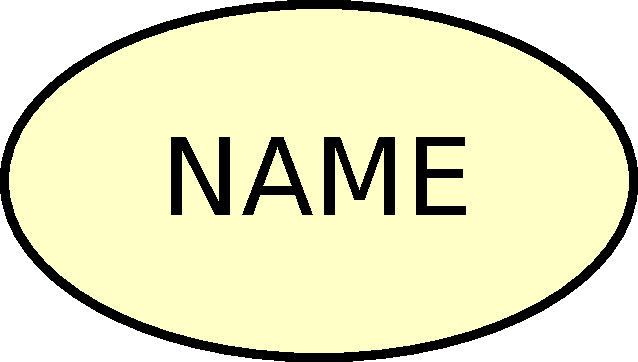
\includegraphics[scale = 0.3]{le_images/unspecified}
  \caption{The \PD glyph for \glyph{unspecified entity}.}
  \label{fig:unspecified}
\end{figure}

\subsubsection{Glyph: \glyph{Macromolecule}}
\label{sec:macromolecule}

Many biological processes involve \emph{macromolecules}: biochemical substances that are built up from the covalent linking of pseudo-identical units.  Examples of macromolecules include proteins, nucleic acids (RNA, DNA), and polysaccharides (glycogen, cellulose, starch, etc.).  Attempting to define a separate glyph for all of these different molecules would lead to an explosion of symbols in SBGN, so instead, \SBGNPDLone defines only one glyph for all macromolecules.  The same glyph is to be used for a protein, a nucleic acid, a complex sugar, and so on.  The exact nature of a particular macromolecule in a map is then clarified using its label and decorations, as will become clear below.  A \glyph{macromolecule} is represented by a rectangular container with rounded corners, as illustrated in \fig{macromolecule}. 

\begin{figure}[H]
  \centering
  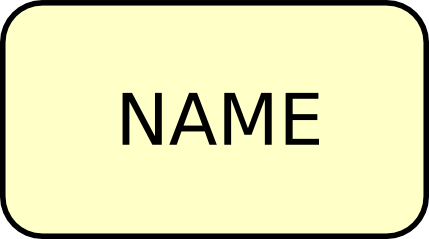
\includegraphics[width = 1.25in]{le_images/macromolecule-plain}
  \caption{The \PD glyph for \glyph{macromolecule}.}
  \label{fig:macromolecule}
\end{figure}

Examples of \glyph{macromolecules} are presented in \fig{macromolecule-examples}.

\begin{figure}[H]
  \centering
  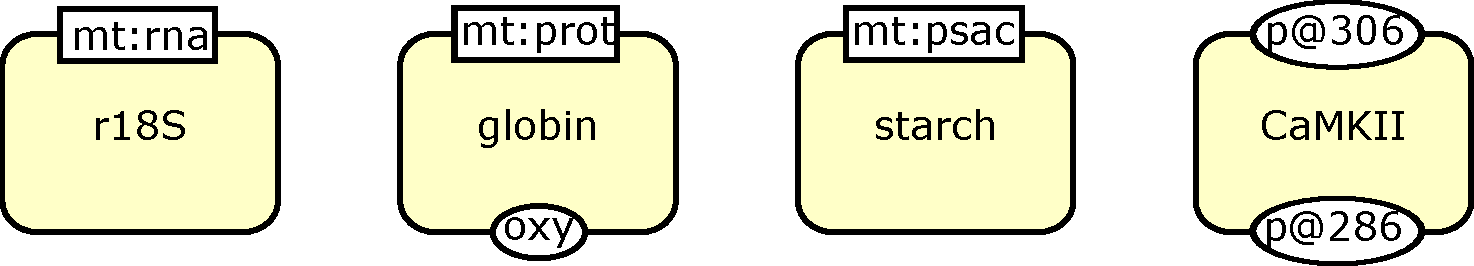
\includegraphics[scale = 0.5]{le_images/macromolecule-examples}
  \caption{Examples of \glyph{macromolecules}. From left to right: the macromolecule of 18S ribosomal RNA, globin (a protein) in the oxygenated state, a molecule of starch (polymer of glucose), calcium calmodulin kinase 2 phosphorylated on threonine 286 and 306.}
  \label{fig:macromolecule-examples}
\end{figure}


\subsubsection{Glyph: \glyph{Simple chemical}}
\label{sec:simpleChemical}

In SBGN \PDs, a simple chemical is defined as the opposite of a macromolecule (\sect{macromolecule}): it is a chemical compound that is \emph{not} formed by the covalent linking of pseudo-identical residues.  Examples of simple chemicals are an atom, a monoatomic ion, a salt, a radical, a solid metal, a crystal, etc. A \glyph{simple chemical} is represented by a circular
container, as depicted in \fig{simpleChemical}. To avoid confusion with the Unspecified Entity (\ref{sec:unspecifiedEntity}), this glyph must remain a circle and cannot be deformed into an ellipse.

\begin{figure}[H]
  \centering
  
\includegraphics[scale = 0.3]{le_images/simpleChemical}
  \caption{The \PD glyph for \glyph{simple chemical}.}
  \label{fig:simpleChemical}
\end{figure}

Examples of \glyph{simple chemicals} are presented in \fig{simpleChemical-examples}.

\begin{figure}[H]
  \centering
  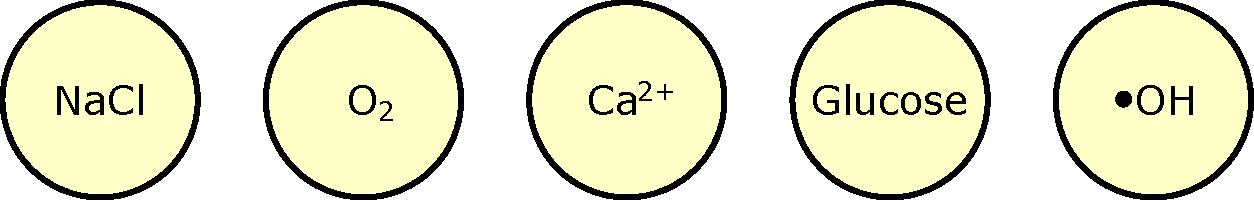
\includegraphics[scale = 0.5]{le_images/simpleChemical-examples}
  \caption{Examples of \glyph{simple chemicals}. From left to right: sodium chloride (a salt), dioxygene (a elemental molecule), calcium ion, glucose (an heteroatomics molecule), hydroxyl radical.}
  \label{fig:simpleChemical-examples}
\end{figure}

\subsubsection{Glyph: \glyph{Nucleic acid feature}}
\label{sec:genetic}

The \emph{Nucleic acid feature} construct in SBGN is meant to represent a fragment of a macromolecule carrying genetic information.  A common use for this construct is to represent a gene or a transcript.  The label of this EPN and its \emph{units of information} (see \sect{unitInfo}) are often important for making the purpose clear to the reader of a map. A \glyph{nucleic acid feature} is represented by a rectangular container whose bottom half has rounded corners, as shown in \fig{genetic}. This design reminds that we are fundamentally dealing with a unit of information, but this information is carried by a macromolecule.

\begin{figure}[H]
  \centering
  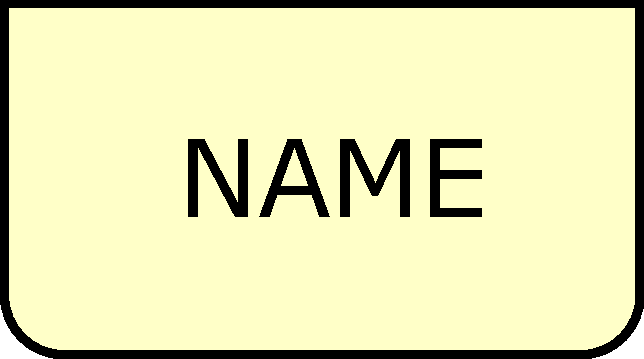
\includegraphics[width = 1.25in]{le_images/genetic}
  \caption{The \PD glyph for \glyph{nucleic acid feature}.} 
  \label{fig:genetic}
\end{figure}

Examples of \glyph{nucleic acid features} are presented in \fig{NucAcidFeat-examples}.

\begin{figure}[H]
  \centering
  \includegraphics[scale = 0.5]{le_images/NucAcidFeat-examples}
  \caption{Examples of \glyph{nucleic acid features}. From left to right: gene coding for the 18S ribosomal RNA, gene coding for $\alpha$1-globin, messenger RNA coding for $\alpha$-globin, nuclear factor 1 binding site on the promoter of $\alpha$1-globin gene.}
  \label{fig:NucAcidFeat-examples}
\end{figure}

\subsubsection{Glyph: \glyph{Complex}}\label{sec:complex}

A \glyph{complex} node represents a biochemical entity composed of other biochemical entities, whether macromolecules, simple chemicals, multimers, or other complexes. The resulting entity may have its own identity, properties and function in an SBGN map. A \glyph{complex} possesses its own container box surrounding the juxtaposed container boxes of its components.  This container box is a rectangle with cut-corners (an octagonal box with sides of two different lengths).  The size of the cut-corners are adjusted so that there is no overlap between the container and the components.  The container boxes of the components must not overlap.

\begin{figure}[H]
  \centering
  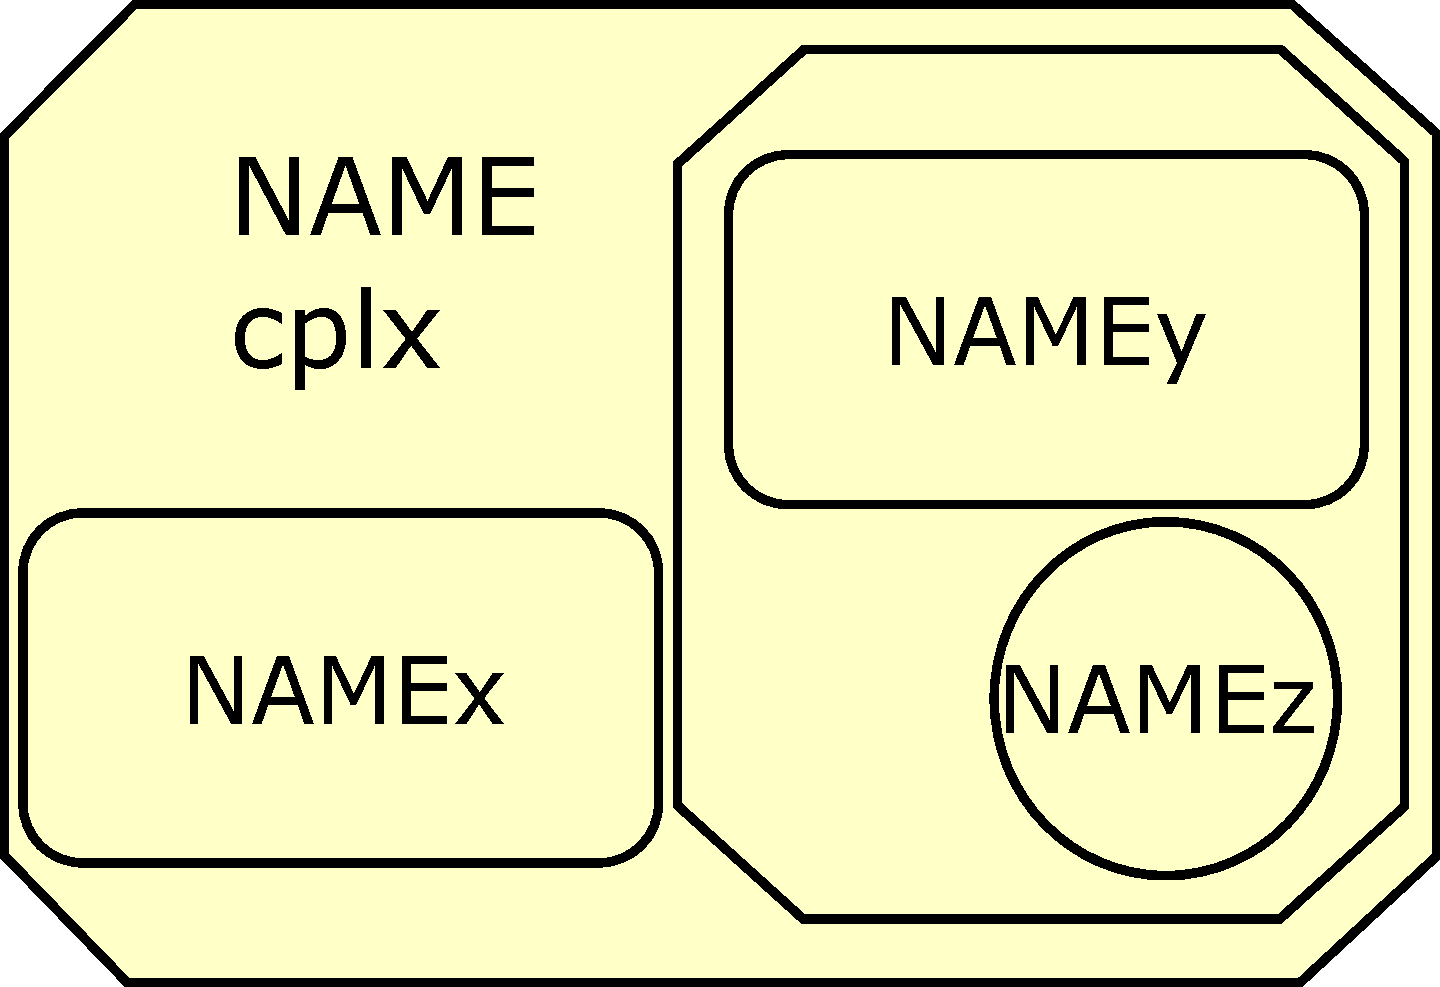
\includegraphics[scale = 0.3]{le_images/complex}
  \caption{The \PD glyph for \glyph{complex}.}
  \label{fig:complex}
\end{figure}


Examples of \glyph{complexes} are presented in \fig{complex-examples}.

\begin{figure}[H]
  \centering
  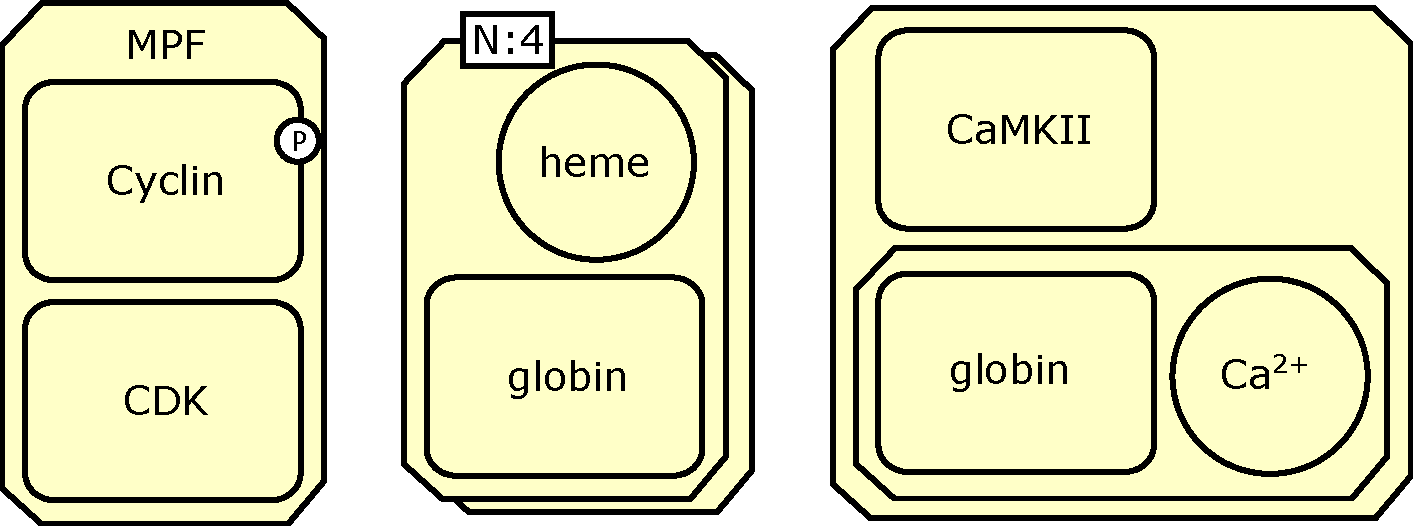
\includegraphics[scale = 0.5]{le_images/complex-examples}
  \caption{Examples of \glyph{complexes}. From left to right: complex between phosphorylated cyclin and CDK2 forming the maturation promoting factor in yeast, a tetramer of complexes between globin and heme, and a complex between calcium-calmodulin kinase II and another complex, itself formed of calmodulin and calcium.}
  \label{fig:complex-examples}
\end{figure}

\subsubsection{Glyph: \glyph{Empty Set}}
\label{sec:sourceSink}

It is useful to have the ability to represent the creation of an entity or
a state from an unspecified source, that is, from something that one does
not need or wish to make precise.  For instance, in a model where the
production of a protein is represented, it may not be desirable to
represent all of the amino acids, sugars and other metabolites used, or the
energy involved in the protein's creation.  Similarly, we may not wish to
bother representing the details of the destruction or decomposition of some
biochemical species into a large number of more primitive entities,
preferring instead to simply say that the species ``disappears into a
sink''.  Yet another example is that one may need to represent an input
(respectively, output) into (resp. from) a compartment without explicitly
representing a transport process from a source (resp. to a target).

For these and other situations, SBGN defines a glyph for explicitly
representing the involvement of an unspecified source or sink. A \glyph{source} or \glyph{sink} is represented by the mathematical symbol for ``empty
set'', that is, a circle crossed by a bar linking the upper-right and
lower-left corners of an invisible square drawn around the circle ($\emptyset$).
\fig{sourceSink} illustrates this. Each source or sink node should be linked to one
and only one arc in a map. The symbol
used in SBGN is borrowed from the mathematical symbol for ``empty set'',
but it is important to note that it does not actually represent a true
absence of everything or a physical void---it represents the absence of the
corresponding structures in the model, that is, the fact that these sources
or sinks are conceptually outside the scope of the map. 

\begin{figure}[H]
  \centering
  
\includegraphics[scale = 0.3]{le_images/sourceSink}
  \caption{The \glyph{source} and \glyph{sink} glyphs.}
  \label{fig:sourceSink}
\end{figure}


\subsubsection{Glyph: \glyph{Perturbing agent}}
\label{sec:perturbing agent}
 
Biochemical networks can be affected by external influences.  Those
influences can be the effect of well-defined physical perturbing agents, such as a light
pulse or a change in temperature; they can also be more complex and not
well-defined phenomena, for instance the outcome of a biological process, an experimental
setup, or a mutation.  For these situations, SBGN provides the
\glyph{perturbing agent} glyph. It is an EPN, and represents the amount to perturbing agent applied to a process. A \glyph{perturbing agent} is represented by a modified hexagon
having two opposite concave faces, as illustrated in \fig{perturbing agent}.

\begin{figure}[H]
  \centering
  
\includegraphics[scale = 0.3]{le_images/perturbing_agent}
  \caption{The \PD glyph for \glyph{perturbing agent}.}
  \label{fig:perturbing agent}
\end{figure}

\subsubsection{Glyph: \glyph{Multimer}}
\label{sec:multimer}

As its name implies, a multimer is an aggregation of multiple identical or pseudo-identical entities held together by non-covalent bonds. Thus, they are distinguished from polymers by the fact that the latter involve covalent bonds, and should be represented by \glyph{macromolecules}. Here \emph{pseudo-identical} refers to the possibility that the entities differ chemically but retain some common global characteristic, such as a structure or function, and so can be considered identical within the context of the SBGN \PD.  An example of this are the homologous subunits in a hetero-oligomeric receptor. SBGN \PD accepts multimers of \glyph{simple chemical} (\sect{simpleChemical}), \glyph{macromolecule} (\sect{macromolecule}), \glyph{nucleic acid feature} (\sect{genetic}) or \glyph{complex} (\sect{complex}). A \glyph{multimer} is represented by two identical containers shifted horizontally and vertically and stacked one on top of the other as illustrated in \fig{multimer}.

\begin{figure}[H]
  \centering
  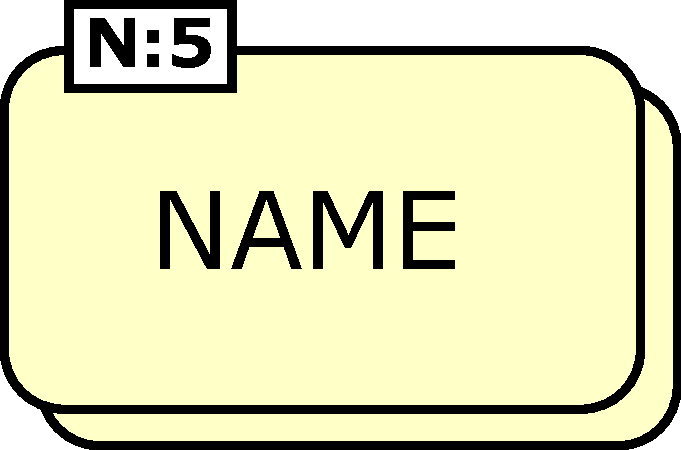
\includegraphics[scale = 0.3]{le_images/multimer}
  \caption{The \PD glyph for \glyph{multimer}. }
  \label{fig:multimer}
\end{figure}

Examples of \glyph{multimers} are presented in \fig{multimer-examples}.

\begin{figure}[H]
  \centering
  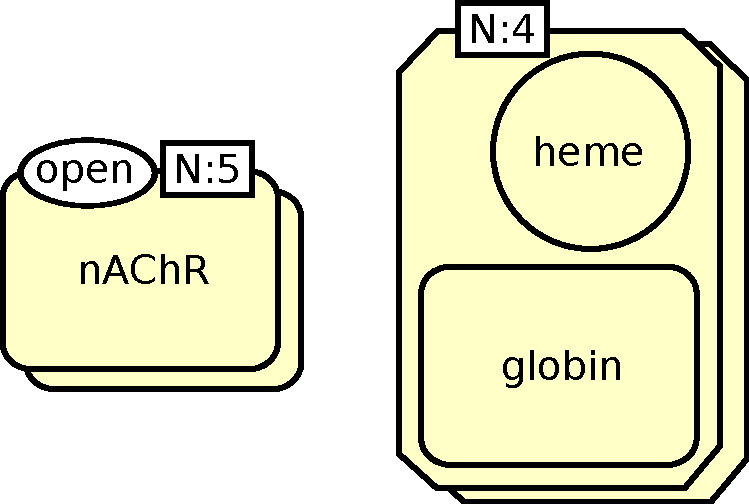
\includegraphics[scale = 0.5]{le_images/multimer-examples}
  \caption{Examples of \glyph{multimers}. From left to right: pentameric nicotinic receptor in the open state, tetramer of oxygenated globin.}
  \label{fig:multimer-examples}
\end{figure}


\subsection{Decorations of the entity pool nodes}\label{sec:decorations}

SBGN \PD provides glyphs that decorate other glyphs, providing additional information that may be useful to the reader. These can provide annotation (\hyperref[sec:unitInfo]{\glyph{unit of information}}), state information (\hyperref[sec:stateVariable]{\glyph{state variable}}) or indicate duplication of entity pool nodes (\hyperref[sec:cloneMarker]{\glyph{clone marker}}).

\subsubsection{Glyph: \glyph{Unit of information}}
\label{sec:unitInfo}

When representing biological entities, it is often necessary to convey some abstract information about the entity's function that is not related to its role in the map.  The \glyph{unit of information} is a decoration that can be used in this situation to add information to an EPN.  Some example uses include: characterizing a logical part of an entity such as a functional domain (a binding domain, a catalytic site, a promoter, etc.), or the information encoded in the entity (an exon, an open reading frame, etc.).  A \glyph{unit of information} can also convey information about the physical environment, or the specific type of biological entity it is decorating. A \glyph{unit of information} is represented by a rectangle overlapping the border of the \glyph{EPN} being annotated.

The label carried by \glyph{unit of information} defines the information it carries.  For certain predefined types of information having controlled vocabularies associated with them, SBGN defines specific prefixes that must be included in the label to indicate the type of information in question.  The controlled vocabularies predefined in \SBGNPDLone are described in \sect{CVs}.

\begin{figure}[H]
  \centering
  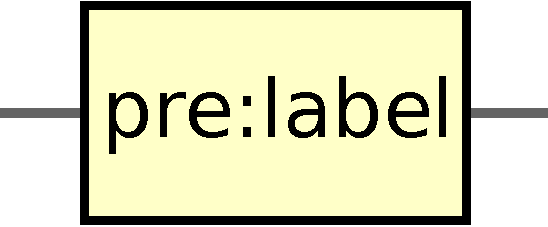
\includegraphics[scale = 0.3]{le_images/unitInformation}
  \caption{The \PD glyph for \glyph{unit of information}.}
  \label{fig:unitInfo}
\end{figure}

\subsubsection{Glyph: \glyph{State variable}}
\label{sec:stateVariable}

Many biological entities, such as molecules, can exist in different \emph{states}, meaning different physical or informational configurations.  These states can arise for a variety of reasons.  For example, macromolecules can be subject to post-synthesis modifications, wherein residues of the macromolecules (amino acids, nucleosides, or glucid residues) are modified through covalent linkage to other chemicals.  Other examples of states are alternative conformations as in the closed/open/desensitized conformations of a transmembrane channel, and the active/inactive forms of an enzyme.

SBGN provides a means of associating one or more \glyph{state variables} with an entity; each such variable can be used to represent a dimension along which the state of the overall entity can vary.  When an entity can exist in different states, the state of the whole entity (\ie the SBGN object) can be described by the current values of all its \glyph{state variables}, and the values of the \glyph{state variables} of all its possible components, recursively. A \glyph{state variable} is represented by an elliptical container overlapping the border of the \glyph{EPN} being annotated.

\begin{figure}[H]
  \centering
  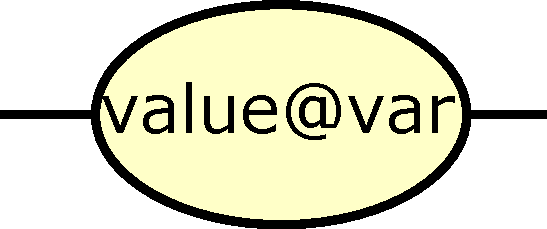
\includegraphics[scale = 0.3, trim = 0 0 0 0.25in]{le_images/stateVariable}
  \caption{The \PD glyph for \glyph{state variable}.}
  \label{fig:state-var}
\end{figure}
 
A \glyph{state variable} does not necessarily have to be Boolean-valued.  For example, an ion channel can possess several conductance states; a receptor can be inactive, active and desensitized; and so on.  As another example, a \glyph{state variable} ``ubiquitin'' could also carry numerical values corresponding to the number of ubiquitin molecules present in the tail.  However, in all cases, a \glyph{state variable} on an EPN can only take \emph{one} defined value.  Further, an EPN's \glyph{state variable} should always be displayed and always set to a value.  An ``empty'' \glyph{state variable} is a \glyph{state variable} that is set to the value ``unset'', it is not a \glyph{state variable} with no value. Note that the value ``unset'' is \emph{not} synonymous to ``any value'' or ``unknown value''.



\subsubsection{Glyph: \glyph{Clone marker}}
\label{sec:cloneMarker}

It is sometimes necessary to represent the same \glyph{EPN} several times. Otherwise, the resulting graph is so tightly connected that the map becomes unreadable. An example would be the representation of currency molecules such as ATP. However, we must indicate the fact, so that a reader knows the processes involving this particular glyph are not the only processes involving the \glyph{EPN}. If an \glyph{EPN} is duplicated on a map, we therefore mark all its graphical reprensation with a \glyph{clone marker} auxiliary unit.  This marker provides the reader with a visual indication that this node has been cloned, and that at least one other occurrence of the \glyph{EPN} can be found in the map (or in a submap; see \sect{submap}).  The clone marker takes two forms, simple and labeled, depending on whether the node being cloned can carry state variables. Note that an \glyph{EPN} belongs to a single compartment. If two glyphs labelled ``X'' are located in two different compartments, such as ATP in cytosol and ATP in mitochondrial lumen, they represent different \glyph{EPNs}, and therefore do not need to be marked as cloned (and if they are, they are not part of the same clone).

The simple (unlabeled) \glyph{clone marker} is a portion of the surface of an \glyph{EPN} that has been modified visually through the use of a different shade, texture, or color.  \fig{simpleCloneMarker} illustrates this. The \glyph{clone marker} occupies the lower part of the \glyph{EPN}. The filled area must be smaller than the unfilled one.

\begin{figure}[H]
  \centering
  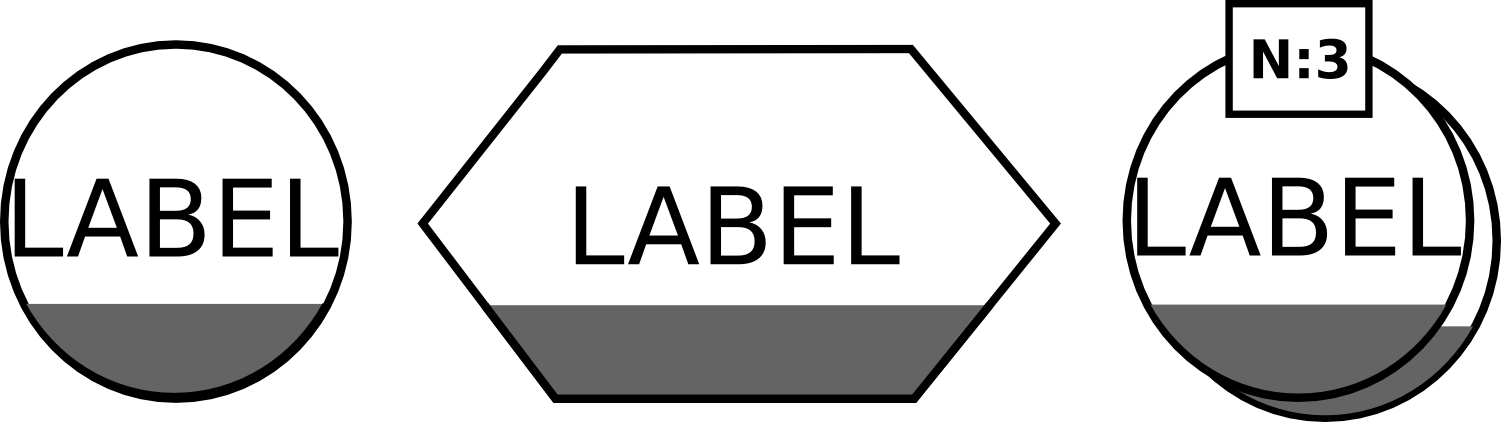
\includegraphics[scale = 0.3]{le_images/simpleCloneMarker}
  \caption{The \PD glyph for \glyph{simple clone marker} applied to a \glyph{simple chemical}}
  \label{fig:simpleCloneMarker}
\end{figure}

Unlike the \glyph{simple clone marker}, the \glyph{labeled clone marker} includes (unsurprisingly, given its name) an identifying label that can be used to identify equivalent clones elsewhere in the map.  This is particularly useful for stateful \glyph{EPNs}, because these can have a large number of state variables displayed and therefore may be difficult to visually identify as being identical. The filled area must be smaller than the unfilled one, but the be large enough to have a height larger than the \glyph{clone marker}'s label (cf below).

\begin{figure}[H]
  \centering
  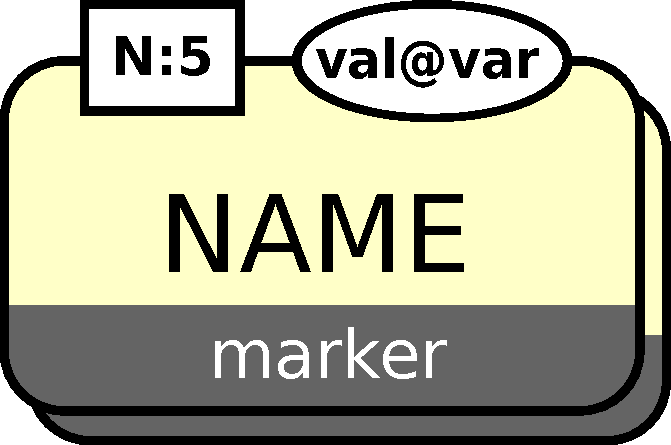
\includegraphics[scale = 0.3]{le_images/labeledCloneMarker}
  \caption{The \PD glyph for \glyph{labeled clone marker} applied to a \glyph{multimer} of  \glyph{macromolecules}.}
  \label{fig:labeledCloneMarker}
\end{figure}


\subsubsection{Glyph: \glyph{Clone marker}}
\label{sec:cloneMarker}

It is sometimes necessary to represent the same \glyph{EPN} several times. Otherwise, the resulting graph is so tightly connected that the map becomes unreadable. An example would be the representation of currency molecules such as ATP. However, we must indicate the fact, so that a reader knows the processes involving this particular glyph are not the only processes involving the \glyph{EPN}. If an \glyph{EPN} is duplicated on a map, we therefore mark all its graphical reprensation with a \glyph{clone marker} auxiliary unit.  This marker provides the reader with a visual indication that this node has been cloned, and that at least one other occurrence of the \glyph{EPN} can be found in the map (or in a submap; see \sect{submap}).  The clone marker takes two forms, simple and labeled, depending on whether the node being cloned can carry state variables. Note that an \glyph{EPN} belongs to a single compartment. If two glyphs labelled ``X'' are located in two different compartments, such as ATP in cytosol and ATP in mitochondrial lumen, they represent different \glyph{EPNs}, and therefore do not need to be marked as cloned (and if they are, they are not part of the same clone).

The simple (unlabeled) \glyph{clone marker} is a portion of the surface of an \glyph{EPN} that has been modified visually through the use of a different shade, texture, or color.  \fig{simpleCloneMarker} illustrates this. The \glyph{clone marker} occupies the lower part of the \glyph{EPN}. The filled area must be smaller than the unfilled one.

\begin{figure}[H]
  \centering
  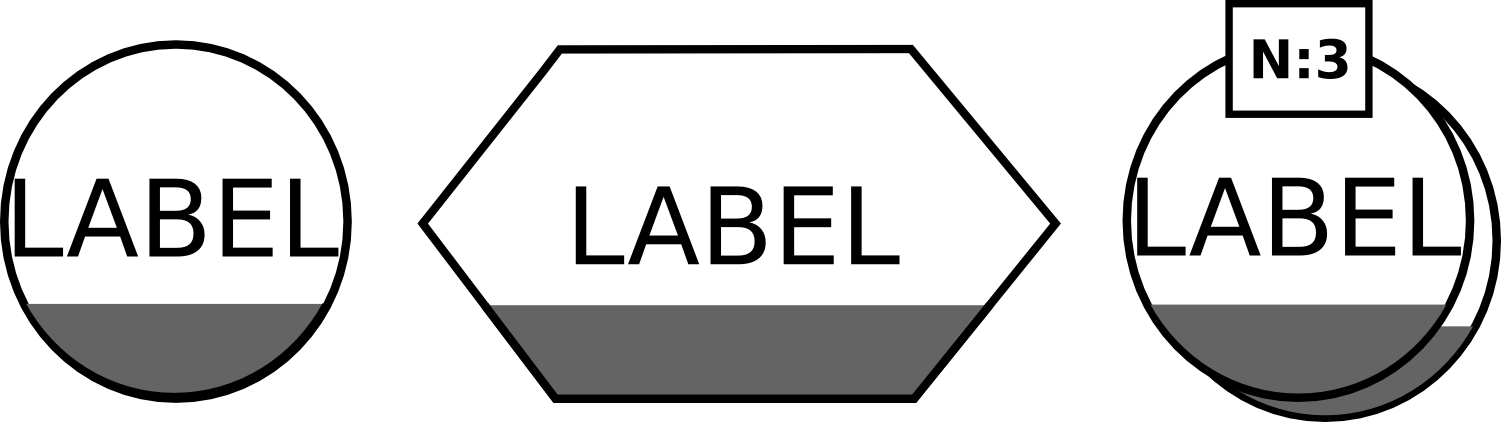
\includegraphics[scale = 0.3]{le_images/simpleCloneMarker}
  \caption{The \PD glyph for \glyph{simple clone marker} applied to a \glyph{simple chemical}}
  \label{fig:simpleCloneMarker}
\end{figure}

Unlike the \glyph{simple clone marker}, the \glyph{labeled clone marker} includes (unsurprisingly, given its name) an identifying label that can be used to identify equivalent clones elsewhere in the map.  This is particularly useful for stateful \glyph{EPNs}, because these can have a large number of state variables displayed and therefore may be difficult to visually identify as being identical. The filled area must be smaller than the unfilled one, but the be large enough to have a height larger than the \glyph{clone marker}'s label (cf below).

\begin{figure}[H]
  \centering
  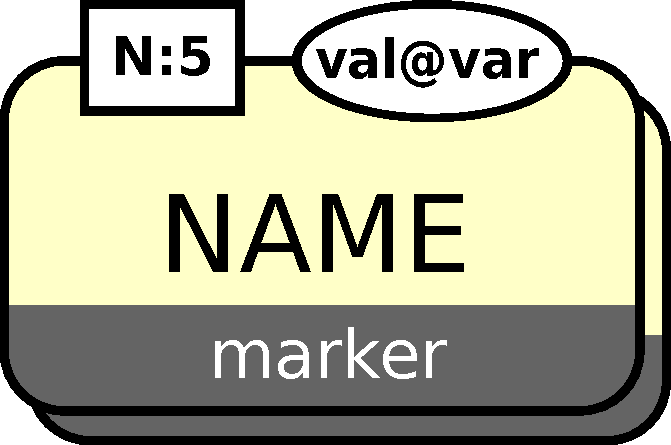
\includegraphics[scale = 0.3]{le_images/labeledCloneMarker}
  \caption{The \PD glyph for \glyph{labeled clone marker} applied to a \glyph{multimer} of  \glyph{macromolecules}.}
  \label{fig:labeledCloneMarker}
\end{figure}


\subsubsection{Controlled vocabularies used in \SBGNPDLone}\label{sec:CVs}

Some glyphs in SBGN \PDs can be enriched with particular kinds of textual annotations conveying information relevant to the purpose of the glyph.  These annotations are \glyph{units of information} (\sect{unitInfo}) or \glyph{state variables}  (\sect{stateVariable}).  An example is the case of multimers, which can carry a \glyph{unit of information} conveying the number of monomers composing the multimer.  Other cases are described throughout the rest of this chapter.

In the rest of this section, we describe the controlled vocabularies (CVs) used in \SBGNPDLone.  They cover the following categories of information: an EPN's material type, an EPN's conceptual type, covalent modifications on macromolecules, the physical characteristics of compartments, and cardinality (\eg of multimers).  In each case, some CV terms are predefined by SBGN. With the exception of covalent modifications, the controlled vocabulary terms contained in \glyph{units of information} or \glyph{state variables} must be prefixed to indicate the type of information being expressed.  Authors may use other CV values not listed here, but in such cases, they should explain the term's meanings in a figure legend or other text accompanying the map.

\subsubsection{Entity pool node material types}
\label{sec:material-types-cv}

The material type of an EPN indicates its chemical structure.  A list of common material types is shown in \tab{material-types-cv}, but others are possible.  The values are to be taken from the \sbo (\cite{Courtot:2011}, \sbourl), specifically from the branch \emph{material entity} under \emph{physical entity representation}.  The labels are defined by \SBGNPDLone.

\begin{table}[h]
  \centering
  \begin{tabular}{l>{\ttfamily}l>{\ttfamily}l}
    \toprule
    \textbf{Name}              & \textbf{\rmfamily Label} & \textbf{\rmfamily SBO term} \\
    \midrule
    Non-macromolecular ion     & mt:ion  & SBO:0000327\\
    Non-macromolecular radical & mt:rad  & SBO:0000328\\
    Ribonucleic acid           & mt:rna  & SBO:0000250\\
    Deoxribonucleic acid       & mt:dna  & SBO:0000251\\
    Protein                    & mt:prot & SBO:0000297\\
    Polysaccharide             & mt:psac & SBO:0000249\\
    \bottomrule
  \end{tabular}
  \caption{A sample of values from the \emph{material types} controlled
    vocabulary (\sect{material-types-cv}).}
  \label{tab:material-types-cv}
\end{table}


\subsubsection{Entity pool node conceptual types}
\label{sec:conceptual-types-cv}

An EPN's \emph{conceptual type} indicates its function within the context of a given \PD.  
In contrast to the \emph{material types}, the \emph{conceptual types} are not about physical composition, but about functional roles.  For example, a strand of RNA is a physical artifact, but its use as messenger RNA is a role.

A list of common conceptual types is shown in \tab{conceptual-types-cv}, but others are possible.  The values are to be taken from the \sbo (\sbourl), specifically from the branch \emph{functional entity} under \emph{physical entity representation}). 

\begin{table}[h]
  \centering
  \begin{tabular}{l>{\ttfamily}l>{\ttfamily}l}
    \toprule
    \textbf{Name}              & \textbf{\rmfamily Label} & \textbf{\rmfamily SBO term} \\
    \midrule
    Gene                      & ct:gene   & SBO:0000243\\
    Transcription start site  & ct:tss    & SBO:0000329\\
    Gene coding region        & ct:coding & SBO:0000335\\
    Gene regulatory region    & ct:grr    & SBO:0000369\\
    Messenger RNA             & ct:mRNA   & SBO:0000278\\
    \bottomrule
  \end{tabular}
  \caption{A sample of values from the \emph{conceptual types} vocabulary
    (\sect{conceptual-types-cv}).}
  \label{tab:conceptual-types-cv}
\end{table}


\subsubsection{Macromolecule covalent modifications}
\label{sec:covalent-mod-cv}

A common reason for the introduction of state variables (\sect{stateVariable}) on an entity is to allow access to the configuration of possible covalent modification sites on that entity.  For instance, a macromolecule may have one or more sites where a phosphate group may be attached; this change in the site's configuration (\ie being either phosphorylated or not) may factor into whether, and how, the entity can participate in different processes.  Being able to describe such modifications in a consistent fashion is the motivation for the existence of SBGN's covalent modifications controlled vocabulary.  

\tab{covalent-mod-cv} lists a number of common types of covalent modifications.  The most common values are defined by the \sbo in the branch \emph{addition of a chemical group}, under \emph{occuring entity representation}. The labels shown in \tab{covalent-mod-cv} are defined by \SBGNPDLone; for all other kinds of modifications not listed here, the author of a \PD must create a new label (and should also describe the meaning of the label in a legend or text accompanying the map).

\begin{table}[h]
  \centering
  \begin{tabular}{l>{\ttfamily}l>{\ttfamily}l}
    \toprule
    \textbf{Name}   & \textbf{\rmfamily Label} & \textbf{\rmfamily SBO term} \\
    \midrule
    Acetylation     & Ac    & SBO:0000215\\
    Glycosylation   & G     & SBO:0000217\\
    Hydroxylation   & OH    & SBO:0000233\\
    Methylation     & Me    & SBO:0000214\\
    Myristoylation  & My    & SBO:0000219\\
    Palmytoylation  & Pa    & SBO:0000218\\
    Phosphorylation & P     & SBO:0000216\\
    Prenylation     & Pr    & SBO:0000221\\
    Protonation     & H     & SBO:0000212\\
    Sulfation       & S     & SBO:0000220\\
    Ubiquitination  & Ub    & SBO:0000224\\
    \bottomrule
  \end{tabular}
  \caption{A sample of values from the \emph{covalent modifications} vocabulary
    (\sect{covalent-mod-cv}).}
  \label{tab:covalent-mod-cv}
\end{table}


\subsubsection{Physical characteristics}
\label{sec:physical-characteristics-cv}

\SBGNPDLone defines a special unit of information for describing certain common physical characteristics.  \tab{physical-characteristics-cv} lists the particular values defined by \SBGNPDLone. 

\begin{table}[h]
  \centering
  \begin{tabular}{l>{\ttfamily}l>{\ttfamily}l}
    \toprule
    \textbf{Name}   & \textbf{\rmfamily Label} & \textbf{\rmfamily SBO term} \\
    \midrule
    Temperature   & pc:T  & SBO:0000147\\
    Voltage       & pc:V  & SBO:0000259\\
    pH            & pc:pH & SBO:0000304\\
    \bottomrule
  \end{tabular}
  \caption{A sample of values from the \emph{physical
      characteristics} vocabulary (\sect{physical-characteristics-cv}).}
  \label{tab:physical-characteristics-cv}
\end{table}


\subsubsection{Cardinality}
\label{sec:cardinality-cv}

\SBGNPDLone defines a special unit of information usable on multimers for describing the number of monomers composing the multimer.  \tab{cardinality-cv} shows the way in which the values must be written.  Note that the value is an positive non-zero integer, and not (for example) a range.  There is at present no provision in \SBGNPDLone for specifying a range in this context because it leads to problems of entity identifiability.

\begin{table}[h]
  \centering
  \begin{tabular}{l>{\ttfamily}l>{\ttfamily}l}
    \toprule
    \textbf{Name}   & \textbf{\rmfamily Label} & \textbf{\rmfamily SBO term} \\
    \midrule
    cardinality    & N:\#  & SBO:0000364\\
    \bottomrule
  \end{tabular}
  \caption{The format of the possible values for the
    \emph{cardinality} unit of information
    (\sect{cardinality-cv}).  Here, \texttt{\#} stands for the
    number; for example, ``\texttt{N:5}''.}
  \label{tab:cardinality-cv}
\end{table}


%%%%%%%%%%%%%%%%%%%%%%%%%%%%%%%%%%%%%%%%%%%%%%%%%%%%%%%%%%%%%%%%%%%%%%
%%%%%%%%%%%%%%%%%%%%%%%%%%%%%%%%%%%%%%%%%%%%%%%%%%%%%%%%%%%%%%%%%%%%%%
%%%%                   Process nodes
%%%%%%%%%%%%%%%%%%%%%%%%%%%%%%%%%%%%%%%%%%%%%%%%%%%%%%%%%%%%%%%%%%%%%%
%%%%%%%%%%%%%%%%%%%%%%%%%%%%%%%%%%%%%%%%%%%%%%%%%%%%%%%%%%%%%%%%%%%%%%

\subsection{Process nodes}\label{sec:PNs}

Process nodes represent processes that transform one or several entity pools into one or several entity pools, identical or different.  \SBGNPDLone defines a generic \glyph{process} (\sect{process}), as well as five more specific ones: the \glyph{omitted process} (\sect{omitted}), the \glyph{uncertain process} (\sect{uncertain}), the \glyph{association} (\sect{association}), the \glyph{dissociation} (\sect{dissociation}), and the \glyph{phenotype} (\sect{phenotype}).

%%%%%%%%%%%%%%%%%%%%%%%%%%%%%%%%%%%%%%%%%%%%%%%%%%%%%%%%%%%%%%%%%%%%%%
%%                     Process
%%%%%%%%%%%%%%%%%%%%%%%%%%%%%%%%%%%%%%%%%%%%%%%%%%%%%%%%%%%%%%%%%%%%%%

\subsubsection{Glyph: \glyph{Process}}
\label{sec:process}

A process is the basic process node in SBGN.  It describes a process that transforms a given set of biochemical entities---macromolecules, simple chemicals or unspecified entities---into another set of biochemical entities.  Such a transformation might imply modification of covalent bonds (conversion), modification of the relative position of constituents (conformational process) or movement from one compartment to another (translocation). A process transforms a set of entity pools (represented by \glyph{EPNs} in \SBGNPDLone) into another set of entity pools. A \glyph{process} is represented by a square box linked to two connectors, small arcs attached to the centers of opposite sides. The consumption (\sect{consumption}) and production (\sect{production}) arcs are linked to the extremities of those connectors. The modulatory arcs (\sect{arcs}) point to the other two sides of the box. A \glyph{process} connected to \glyph{production} arcs on opposite sides is a reversible process. 

\begin{figure}[H]
  \centering
  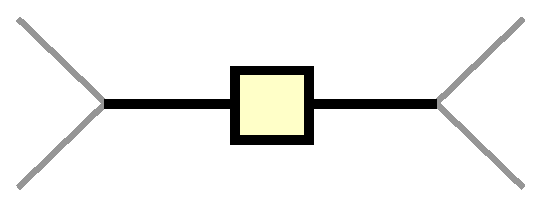
\includegraphics[scale = 0.4]{le_images/process}
  \caption{The \PD glyph for \glyph{process}.}
  \label{fig:process}
\end{figure}

The example in \fig{trans-react} illustrates the use of a \glyph{process} node to represent a reaction between two reactants that generates three products. The stoichiometry for each entity pool involved is 1, and therefore can be omitted.  

\begin{figure}[H]
  \centering
  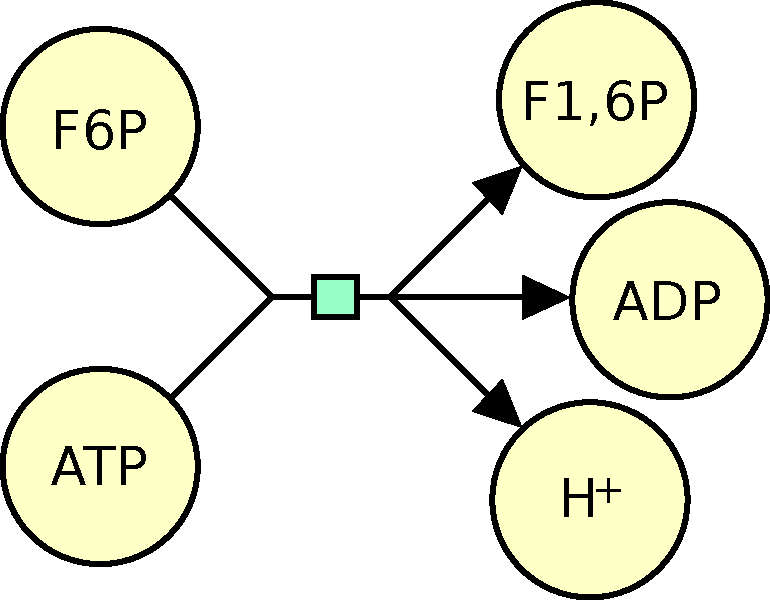
\includegraphics[scale = 0.5]{le_images/process-reaction}
  \caption{Reaction between ATP and fructose-6-phosphate to produce fructose-1,6-biphosphate, ADP and a proton.}
  \label{fig:trans-react}
\end{figure}

The example in \fig{trans-phos} illustrates the use of a \glyph{process} node to represent the phosphorylation of a protein. 

\begin{figure}[H]
  \centering
  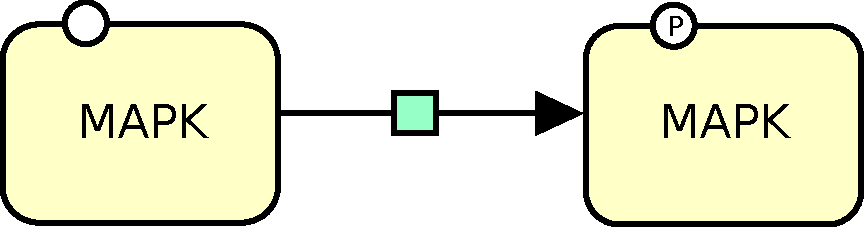
\includegraphics[scale = 0.5]{le_images/process-phosphorylation}
  \caption{Phosphorylation of the protein MAP kinase.}
  \label{fig:trans-phos}
\end{figure}


The example in \fig{trans-trans} illustrates the use of a \glyph{process} node to represent a translocation. The large round-cornered rectangle represents a compartment border (see \sect{compartment}).

\begin{figure}[H]
  \centering
  \includegraphics[scale = 0.5]{le_images/process-translocation}
  \caption{Translocation of calcium ion out of the endoplasmic reticulum. Note that the \glyph{process} does not have to be located on the boundary of the \glyph{compartment}. A \glyph{process} is not attached to any \glyph{compartment}.}
  \label{fig:trans-trans}
\end{figure}

The example in \fig{trans-dim} presents the conversion of two galactoses into a lactose.  Galactoses are represented by only one \glyph{simple chemical}, the cardinality being carried by the \glyph{consumption} arc.

\begin{figure}[H]
  \centering
  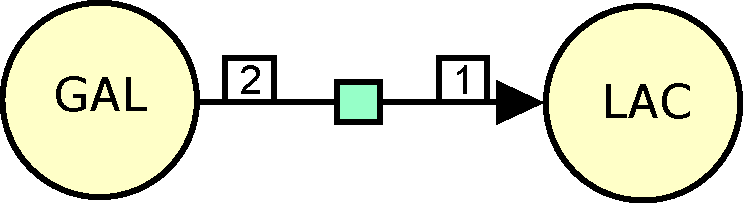
\includegraphics[scale = 0.5]{le_images/process-dimerisation}
  \caption{Conversion of two galactoses into a lactose.}
  \label{fig:trans-dim}
\end{figure}

%%%%%%%%%%%%%%%%%%%%%%%%%%%%%%%%%%%%%%%%%%%%%%%%%%%%%%%%%%%%%%%%%%%%%%
%%                     Omitted Process
%%%%%%%%%%%%%%%%%%%%%%%%%%%%%%%%%%%%%%%%%%%%%%%%%%%%%%%%%%%%%%%%%%%%%%
%\color{blue}
\subsubsection{Glyph: \glyph{Omitted process}}\label{sec:omitted}

Omitted processes are processes that are known to exist, but are omitted from the map for the sake of clarity or parsimony. A single \glyph{omitted process} can represent any number of actual processes. For instance, one may want to represent a long chain of processes leading from one biochemical compound to another, without detailing all steps, but highlighting the fact that this is not a direct transformation.  The \glyph{omitted process} is different from a \glyph{submap} (\sect{submap}). While a \glyph{submap} references to an explicit content, that is hidden in the main map, the \glyph{omitted process} does not ``hide'' anything within the context of the map, and cannot be ``unfolded''. An \glyph{omitted process} is represented by a \glyph{process} in which the square box contains a two parallel slanted lines oriented northwest-to-southeast and separated by an empty space.

\begin{figure}[H]
  \centering
  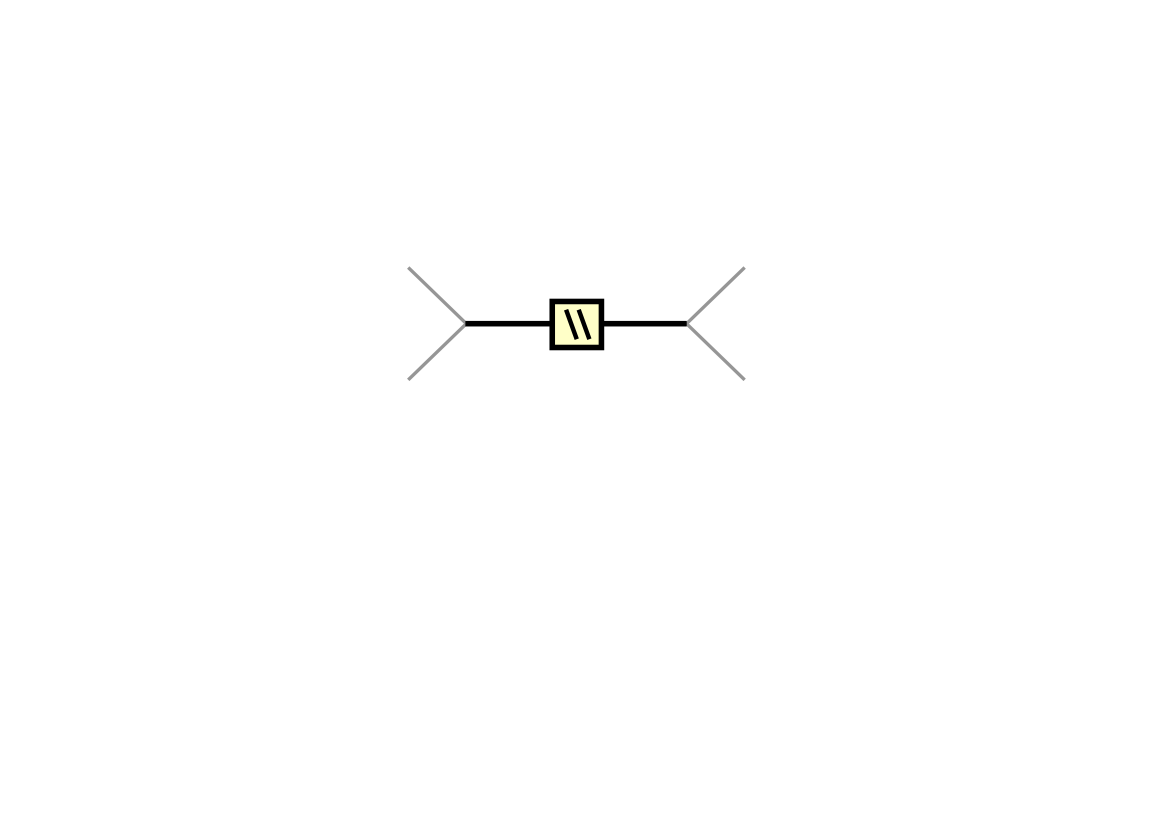
\includegraphics[scale = 0.5]{le_images/omitted}
  \caption{The \PD glyph for \glyph{omitted process}.}
  \label{fig:omitted}
\end{figure}



%%%%%%%%%%%%%%%%%%%%%%%%%%%%%%%%%%%%%%%%%%%%%%%%%%%%%%%%%%%%%%%%%%%%%%
%%                     Uncertain Process
%%%%%%%%%%%%%%%%%%%%%%%%%%%%%%%%%%%%%%%%%%%%%%%%%%%%%%%%%%%%%%%%%%%%%%
%\color{blue}
\subsubsection{Glyph: \glyph{Uncertain process}}\label{sec:uncertain}

Uncertain processes are processes that may not exist. A single \glyph{uncertain process} can represent any number of actual processes. \glyph{Uncertain process} would be used to represent hypothesis, reactions which existence is supported by weak evidence etc. An \glyph{uncertain process} is represented by a \glyph{process} which square box contains a question mark.

\begin{figure}[H]
  \centering
  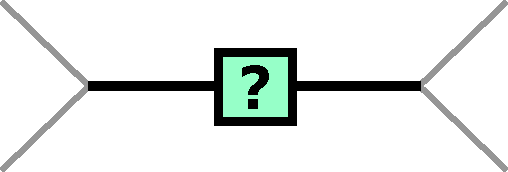
\includegraphics[scale = 0.5]{le_images/uncertain}
  \caption{The \PD glyph for an \glyph{uncertain process}.}
  \label{fig:uncertain}
\end{figure}

%%%%%%%%%%%%%%%%%%%%%%%%%%%%%%%%%%%%%%%%%%%%%%%%%%%%%%%%%%%%%%%%%%%%%%
%%                     Association
%%%%%%%%%%%%%%%%%%%%%%%%%%%%%%%%%%%%%%%%%%%%%%%%%%%%%%%%%%%%%%%%%%%%%%

\subsubsection{Glyph: \glyph{Association}}\label{sec:association}

The association between one or more \glyph{EPNs} represents the non-covalent binding of the biological objects represented by those \glyph{EPNs} into a larger complex. An \glyph{association} between several entities is represented by a filled disc linked to two connectors separated by 180 degrees. The consumption (\sect{consumption}) and production (\sect{production}) arcs are linked to the extremities of those connectors. An \glyph{association} is never reversible, the inverse process being represented by a \glyph{dissociation} (\sect{dissociation}).

\begin{figure}[H]
  \centering
  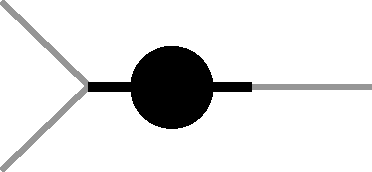
\includegraphics[scale = 0.5]{le_images/association}
  \caption{The \PD glyph for \glyph{association}.}
  \label{fig:association}
\end{figure}

The example in \fig{assoc-cyclin} illustrates the association of cyclin and CDC2 kinase into the Maturation Promoting Factor.

\begin{figure}[H]
  \centering
  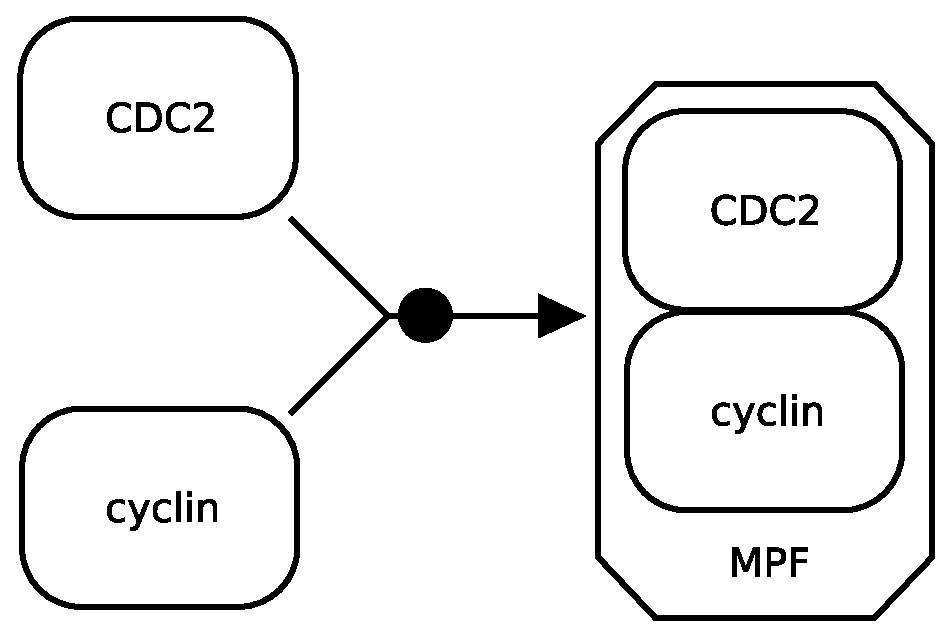
\includegraphics[scale = 0.5]{le_images/association-MPF}
  \caption{Association of cyclin and CDC2 kinase into the Maturation Promoting Factor.}
  \label{fig:assoc-cyclin}
\end{figure}

An \glyph{association} does not necessarily involve components of the same nature. \fig{assoc-unamed} gives an example illustrating the association of a pentameric \glyph{macromolecule} (a nicotinic acetylcholine receptor) with a \glyph{simple chemical} (the local anesthetic chlorpromazin) in an unnamed complex.

\begin{figure}[H]
  \centering
  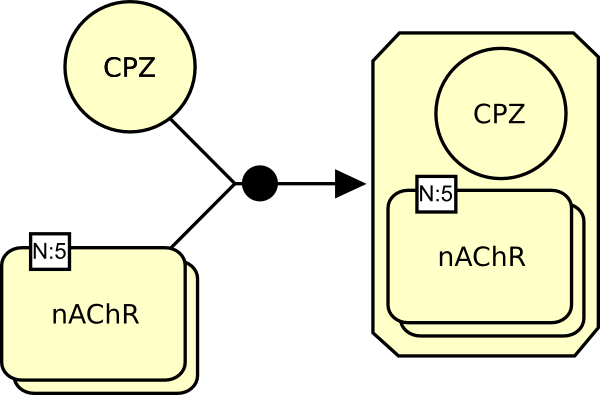
\includegraphics[scale = 0.5]{le_images/association-unamed}
  \caption{The association of a pentameric macromolecule with a simple chemical in an unnamed complex.}
  \label{fig:assoc-unamed}
\end{figure}

An association does not necessarily result in the formation of a \glyph{complex}; it can also produce a \glyph{multimer}. \fig{assoc-multi} gives an example of using the successive formation of an hemoglobin monomer then a tetramer of the resulting complex.

\begin{figure}[H]
  \centering
  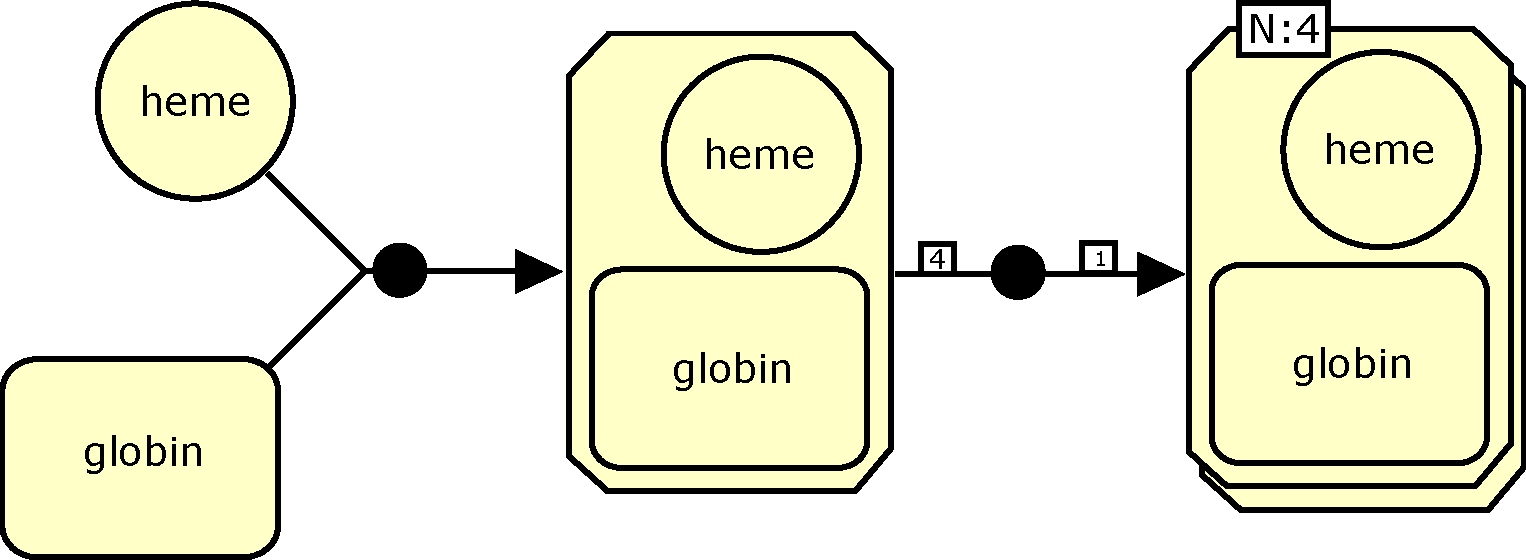
\includegraphics[scale = 0.5]{le_images/association-multimerisation}
  \caption{Formation of hemoglobin.}
  \label{fig:assoc-multi}
\end{figure}


%%%%%%%%%%%%%%%%%%%%%%%%%%%%%%%%%%%%%%%%%%%%%%%%%%%%%%%%%%%%%%%%%%%%%%
%%                     Dissociation
%%%%%%%%%%%%%%%%%%%%%%%%%%%%%%%%%%%%%%%%%%%%%%%%%%%%%%%%%%%%%%%%%%%%%%
%\color{blue}
\subsubsection{Glyph: \glyph{Dissociation}}\label{sec:dissociation}

The dissociation of an \glyph{EPN} into one or more \glyph{EPNs} represents the rupture of a non-covalent binding between the biological entities represented by those \glyph{EPNs}. A \glyph{dissociation} between several entities is represented by two concentric circles. A simple empty disc could be, in some cases, confused with the \glyph{catalysis} (section \sect{catalysis}). Moreover, the existence of two circles reminds the dissociation, by contrast with the filled disc of the \glyph{association} (\sect{association}).

\begin{figure}[H]
  \centering
  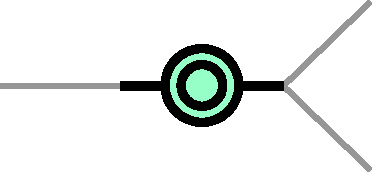
\includegraphics[scale = 0.5]{le_images/dissociation}
  \caption{The \PD glyph for \glyph{dissociation}.}
  \label{fig:dissociation}
\end{figure}

\subsubsection{Glyph: \glyph{Phenotype}}
\label{sec:phenotype}

A biochemical network can generate phenotypes or affect biological
processes.  Such processes can take place at different levels and are
independent of the biochemical network itself.  To represent these
processes in a map, SBGN defines the \glyph{phenotype} glyph, which describes a process consuming nothing and producing nothing, but only modulated. A \glyph{phenotype} is represented by an hexagone, as illustrated in \fig{phenotype}. 

\begin{figure}[H]
  \centering
  
\includegraphics[scale = 0.3]{le_images/phenotype}
  \caption{The \PD glyph for \glyph{phenotype}.}
  \label{fig:phenotype}
\end{figure}

The example in \fig{phenotype-MPF} illustrates the use of a \glyph{phenotype} node to represent cell division, stimulated by the mono-phosphorylated form of the maturation promoting factor (see \sect{stimulation} for the meaning of the open arrowhead). 

\begin{figure}[H]
  \centering
  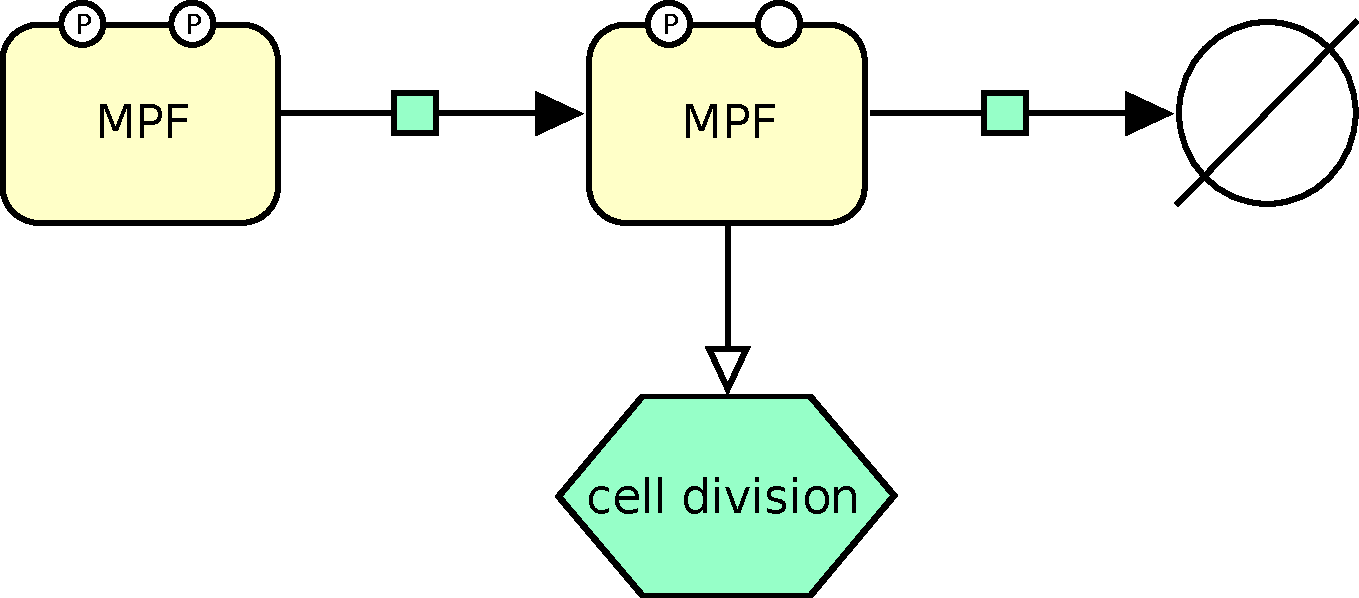
\includegraphics[scale = 0.5]{le_images/phenotype-MPF}
  \caption{Cell division stimulated by MPF.}
  \label{fig:phenotype-MPF}
\end{figure}


%%%%%%%%%%%%%%%%%%%%%%%%%%%%%%%%%%%%%%%%%%%%%%%%%%%%%%%%%%%%%%%%%%%%%%
%%%%%%%%%%%%%%%%%%%%%%%%%%%%%%%%%%%%%%%%%%%%%%%%%%%%%%%%%%%%%%%%%%%%%%
%%%%                  Arcs
%%%%%%%%%%%%%%%%%%%%%%%%%%%%%%%%%%%%%%%%%%%%%%%%%%%%%%%%%%%%%%%%%%%%%%
%%%%%%%%%%%%%%%%%%%%%%%%%%%%%%%%%%%%%%%%%%%%%%%%%%%%%%%%%%%%%%%%%%%%%%

\subsection{Arcs}\label{sec:arcs}

Arcs are lines that link nodes of SBGN together. The symbols attached to their extremities indicate their meaning. \SBGNPDLone defines nine arcs. \glyph{consumption} (\sect{consumption}), \glyph{production} (\sect{production}), \glyph{modulation} (\sect{modulation}), \glyph{stimulation} (\sect{stimulation}), \glyph{catalysis} (\sect{catalysis}), \glyph{inhibition} (\sect{inhibition}), and \glyph{necessary stimulation} (\sect{necessary_stim}) connect \glyph{EPNs} to \glyph{PDs}. \glyph{LogicArc} (\sect{logicArc}) link \glyph{EPNs} and \glyph{logic arcs}.  \glyph{equivalenceArc} (\sect{equivalenceArc}) link nodes to \glyph{tag}. Arcs can take any shape, and are not restricted to segments of straight lines.


%%%%%%%%%%%%%%%%%%%%%%%%%%%%%%%%%%%%%%%%%%%%%%%%%%%%%%%%%%%%%%%%%%%%%%
%%                     Consumption
%%%%%%%%%%%%%%%%%%%%%%%%%%%%%%%%%%%%%%%%%%%%%%%%%%%%%%%%%%%%%%%%%%%%%%

\subsubsection{Glyph: \glyph{Consumption}}
\label{sec:consumption}

\glyph{Consumption} is the arc used to represent the fact that an entity pool is consumed by a process, but is not produced by the process. A \glyph{consumption} is represented by a simple line without particular symbols at its extremities. A cardinality label may be associated with \glyph{consumption} (\sect{consumption}) indicating the stoichiometry of the entity pool node for this process. This label is a number enclosed in a rectangle with one of the long sides adjacent to the consumption arc. Once assigned to one arc connecting to a process node, cardinality should be represented on all \glyph{consumption} and \glyph{production} arcs connected to that process node to avoid misinterpretation. In the case where the stoichiometry of some part of the process is not known, or undefined, a question mark (?) should be used within the cardinality label
of the corresponding arcs.

\begin{figure}[H]
  \centering
  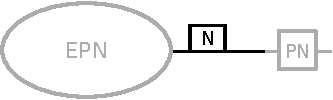
\includegraphics[scale = 0.4]{le_images/consumption}
  \caption{The \PD glyph for \glyph{consumption}.}
  \label{fig:consumption}
\end{figure}


%%%%%%%%%%%%%%%%%%%%%%%%%%%%%%%%%%%%%%%%%%%%%%%%%%%%%%%%%%%%%%%%%%%%%%
%%                     Production
%%%%%%%%%%%%%%%%%%%%%%%%%%%%%%%%%%%%%%%%%%%%%%%%%%%%%%%%%%%%%%%%%%%%%%

\subsubsection{Glyph: \glyph{Production}}\label{sec:production}

\glyph{Production} is the arc used to represent the fact that an entity pool is produced by a process. In the case of a reversible process, the 
\glyph{production} arc also acts as a \glyph{consumption} arc. The target extremity of a \glyph{production} carries a filled arrowhead. A cardinality label can be associated with a \glyph{production} arc indicating the stoichiometry of a process.

\begin{figure}[H]
  \centering
  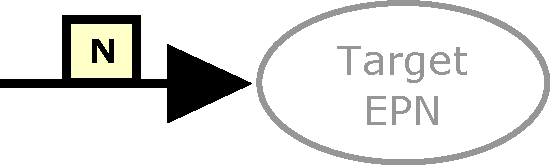
\includegraphics[scale = 0.4]{le_images/production}
  \caption{The \PD glyph for \glyph{production}.}
  \label{fig:production}
\end{figure}

%%%%%%%%%%%%%%%%%%%%%%%%%%%%%%%%%%%%%%%%%%%%%%%%%%%%%%%%%%%%%%%%%%%%%%
%%                     Modulation
%%%%%%%%%%%%%%%%%%%%%%%%%%%%%%%%%%%%%%%%%%%%%%%%%%%%%%%%%%%%%%%%%%%%%%
%\color{blue}
\subsubsection{Glyph: \glyph{Modulation}}\label{sec:modulation}

A modulation affects the flux of a process represented by the target process. Such a modulation can affect the
process \textbf{positively or negatively}, or even both ways depending on the conditions, for instance the concentration of the intervening
participants. A \glyph{modulation} can also be used when one does not know the precise direction of the effect. The target extremity of a \glyph{modulation} carries an empty diamond.

\begin{figure}[H]
  \centering
  
\includegraphics[scale = 0.5]{le_images/modulation}
  \caption{The \PD glyph for \glyph{modulation}.}
  \label{fig:modulation}
\end{figure}

\fig{modul-nico} represents the effect of nicotine on the process converting closed and open states of a nicotinic acetylcholine receptor. High concentrations of nicotine open the receptor while low concentrations can desensitize it without opening. 

\begin{figure}[H]
  \centering
  \includegraphics[scale = 0.5]{le_images/modulation-nAChR}
  \caption{Modulation of nicotinic receptor opening by nicotine.}
  \label{fig:modul-nico}
\end{figure}

%%%%%%%%%%%%%%%%%%%%%%%%%%%%%%%%%%%%%%%%%%%%%%%%%%%%%%%%%%%%%%%%%%%%%%
%%                     Stimulation
%%%%%%%%%%%%%%%%%%%%%%%%%%%%%%%%%%%%%%%%%%%%%%%%%%%%%%%%%%%%%%%%%%%%%%

\subsubsection{Glyph: \glyph{Stimulation}}\label{sec:stimulation}

A stimulation affects \textbf{positively} the flux of a process represented by the target process. This stimulation can be for instance a catalysis or a positive allosteric regulation. Note that \glyph{catalysis} exists independently in SBGN, see \sect{catalysis}. The target extremity of a \glyph{stimulation} carries an empty arrowhead.

\begin{figure}[H]
  \centering
  
\includegraphics[scale = 0.5]{le_images/stimulation}
  \caption{The \PD glyph for \glyph{stimulation}.}
  \label{fig:stimulation}
\end{figure}

The example in \fig{stimulation-reversible} illustrates the use of two \glyph{stimulations} arcs to represent the opposite effects of agonists and inverse agonists on G-protein coupled receptor activity. Agonists stimulate the transition from inactive to active, while inverse agonists stimulate the transition inactive to active.

\begin{figure}[H]
  \centering
  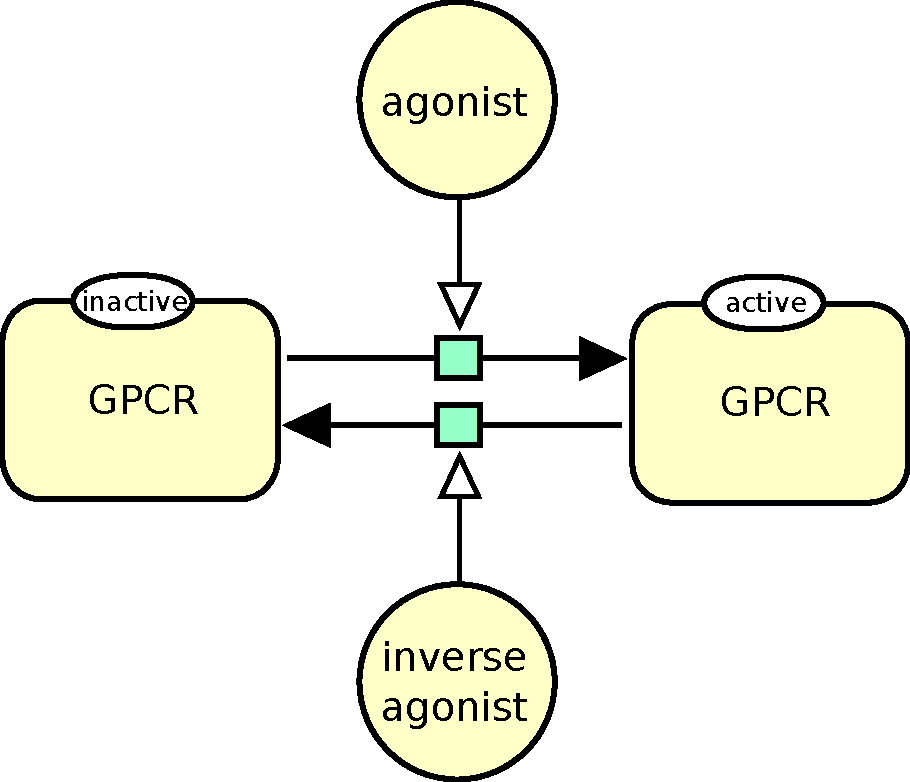
\includegraphics[scale = 0.5]{le_images/stimulation-reversible}
  \caption{Opposite effects of agonists and inverse agonists on GPCRs.}
  \label{fig:stimulation-reversible}
\end{figure}

%%%%%%%%%%%%%%%%%%%%%%%%%%%%%%%%%%%%%%%%%%%%%%%%%%%%%%%%%%%%%%%%%%%%%%
%%                     Catalysis
%%%%%%%%%%%%%%%%%%%%%%%%%%%%%%%%%%%%%%%%%%%%%%%%%%%%%%%%%%%%%%%%%%%%%%
%\color{blue}
\subsubsection{Glyph: \glyph{Catalysis}}\label{sec:catalysis}

A catalysis is a particular case of stimulation, where the effector affects
positively the flux of a process represented by the target process. The positive effect on the process is due to the lowering of the activation energy of a reaction. The target extremity of a \glyph{catalysis} carries an empty circle.

\begin{figure}[H]
  \centering
  
\includegraphics[scale = 0.5]{le_images/catalysis}
  \caption{The \PD glyph for \glyph{catalysis}.}
  \label{fig:catalysis}
\end{figure}

The example in \fig{catalysis-MAPK} illustrates the use of \glyph{catalysis} arc to represent the effect of MAPKK on the phophorylation of MAPK.

\begin{figure}[H]
  \centering
  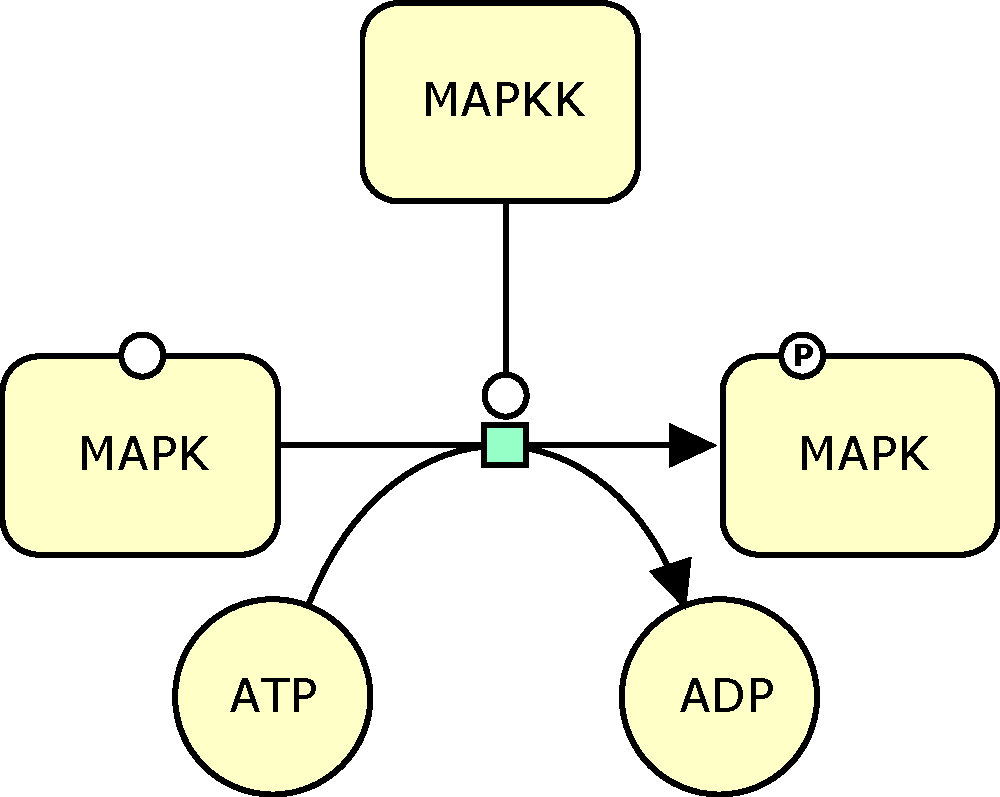
\includegraphics[scale = 0.5]{le_images/catalysis-MAPK}
  \caption{MAPKK catalyses the phosphorylation of MAPK.}
  \label{fig:catalysis-MAPK}
\end{figure}


%%%%%%%%%%%%%%%%%%%%%%%%%%%%%%%%%%%%%%%%%%%%%%%%%%%%%%%%%%%%%%%%%%%%%%
%%                     Inhibition
%%%%%%%%%%%%%%%%%%%%%%%%%%%%%%%%%%%%%%%%%%%%%%%%%%%%%%%%%%%%%%%%%%%%%%

\subsubsection{Glyph: \glyph{Inhibition}}\label{sec:inhibition}
%\color{blue}

An inhibition \textbf{negatively} affects the flux of a process represented by the target process. This inhibition can be for instance a competitive inhibition or an allosteric inhibition. The target extremity of an \glyph{inhibition} carries a bar perpendicular to the arc.

\begin{figure}[H]
  \centering
  
\includegraphics[scale = 0.5]{le_images/inhibition}
  \caption{The \PD glyph for \glyph{inhibition}.}
  \label{fig:inhibition}
\end{figure}




%%%%%%%%%%%%%%%%%%%%%%%%%%%%%%%%%%%%%%%%%%%%%%%%%%%%%%%%%%%%%%%%%%%%%%
%%                     Necessary_Stim
%%%%%%%%%%%%%%%%%%%%%%%%%%%%%%%%%%%%%%%%%%%%%%%%%%%%%%%%%%%%%%%%%%%%%%

\subsubsection{Glyph: \glyph{Necessary stimulation}}\label{sec:necessary_stim}

A necessary stimulation, is one that is necessary for a process to take place. A process modulated by a necessary stimulation can only occur when this necessary stimulation is active. The target extremity of a \glyph{necessary stimulation} carries an open arrow (to remind that it is a \glyph{stimulation}) coming after a larger vertical bar.

\begin{figure}[H]
  \centering
  
\includegraphics[scale = 0.5]{le_images/necessary_stim}
  \caption{The \PD glyph for \glyph{Necessary Stimulation}.}
  \label{fig:Necessary Stimulation}
\end{figure}

The example in \fig{necessary_stim-gene} below describes the transcription of a gene~X, that is the creation of a messenger RNA~X triggered by the gene~X.  The creation of the protein~X is then triggered by the mRNA~X.  (Note that the same example could be represented using the gene as reactant and product, although it is semantically different.)

\begin{figure}[H]
  \centering
  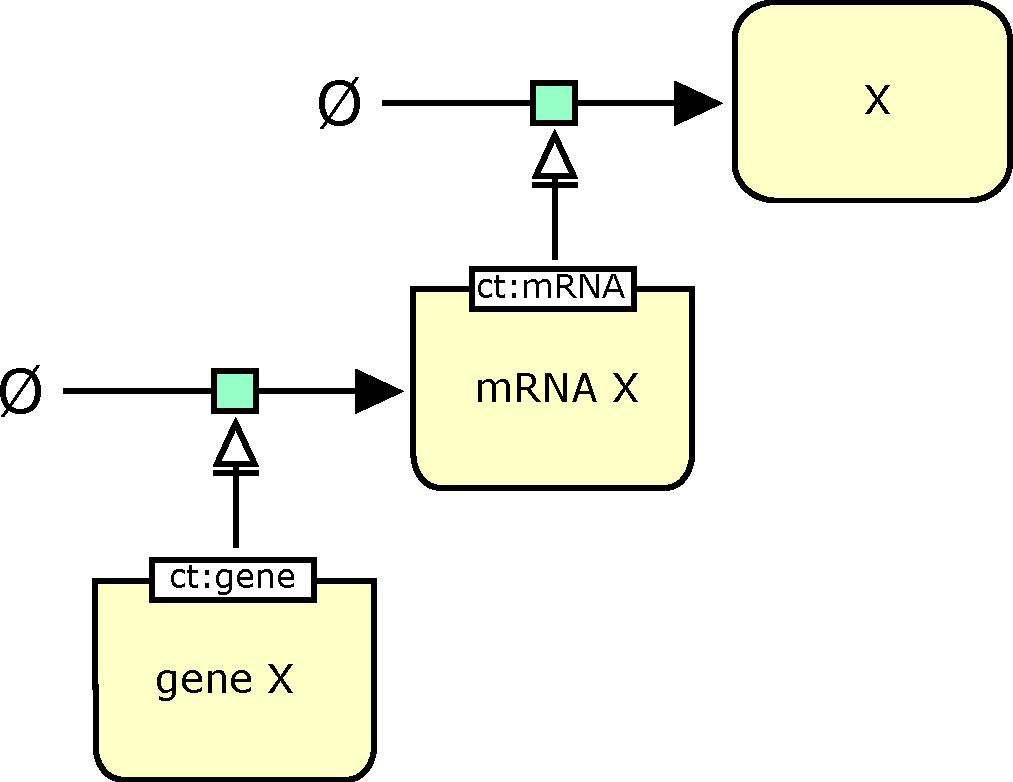
\includegraphics[scale = 0.5]{le_images/necessary_stim-genetic}
  \caption{The creation of a messenger RNA~X triggered by the gene~X.}
  \label{fig:necessary_stim-gene}
\end{figure}


The example in \fig{necessary_stim-calcium} below describes the transport of calcium ions out of the endoplasmic reticulum. Without IP3 receptor, there is not calcium flux, therefore, one cannot use a \glyph{stimulation}. The Necessary Stimulation instead represents this absolute stimulation.

\begin{figure}[H]
  \centering
  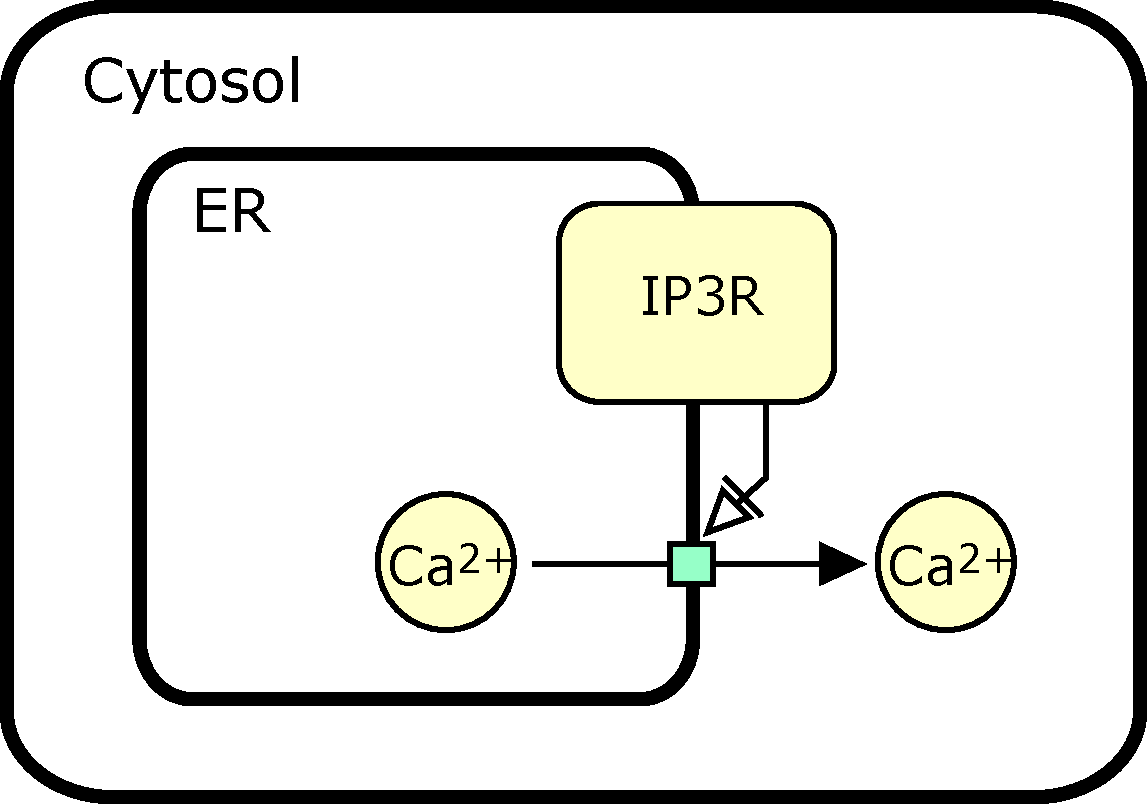
\includegraphics[scale = 0.5]{le_images/necessary_stim-transport}
  \caption{The transport of calcium ions out of the endoplasmic reticulum into the cytosol. Note that IP3R crosses both compartment boundaries. This is allowed, but the Macromolecule should only belong to one of the compartments.}
  \label{fig:necessary_stim-calcium}
\end{figure}


%%%%%%%%%%%%%%%%%%%%%%%%%%%%%%%%%%%%%%%%%%%%%%%%%%%%%%%%%%%%%%%%%%%%%%
%%                     Logic arc
%%%%%%%%%%%%%%%%%%%%%%%%%%%%%%%%%%%%%%%%%%%%%%%%%%%%%%%%%%%%%%%%%%%%%%
%\color{blue}
\subsubsection{Glyph: \glyph{Logic arc} }\label{sec:logicArc}

\glyph{Logic arc} is used to represent the fact that an entity influences the outcome of a logic operator. A \glyph{logic arc} is represented by a simple line without particular symbols at its extremities.

\begin{figure}[H]
  \centering
  
\includegraphics[scale = 0.4]{le_images/logicArc}
  \caption{The \PD glyph for \glyph{logic arc}.}
  \label{fig:logicArc}
\end{figure}

%%%%%%%%%%%%%%%%%%%%%%%%%%%%%%%%%%%%%%%%%%%%%%%%%%%%%%%%%%%%%%%%%%%%%%
%%                     Equivalence Arc
%%%%%%%%%%%%%%%%%%%%%%%%%%%%%%%%%%%%%%%%%%%%%%%%%%%%%%%%%%%%%%%%%%%%%%
%\color{blue}
\subsubsection{Glyph: \glyph{Equivalence arc} }\label{sec:equivalenceArc}

\glyph{Equivalence arc} is the arc used to represent the fact that all entities
marked by a \glyph{tag} are equivalent. An \glyph{equivalence arc} is represented by a simple line without particular symbols at its extremities.

\begin{figure}[H]
  \centering
  
\includegraphics[scale = 0.4]{le_images/equivalence}
  \caption{The \PD glyph for \glyph{Equivalence arc}.}
  \label{fig:equivalence}
\end{figure}



%%%%%%%%%%%%%%%%%%%%%%%%%%%%%%%%%%%%%%%%%%%%%%%%%%%%%%%%%%%%%%%%%%%%%%
%%%%%%%%%%%%%%%%%%%%%%%%%%%%%%%%%%%%%%%%%%%%%%%%%%%%%%%%%%%%%%%%%%%%%%
%%%%                   Logical operators
%%%%%%%%%%%%%%%%%%%%%%%%%%%%%%%%%%%%%%%%%%%%%%%%%%%%%%%%%%%%%%%%%%%%%%
%%%%%%%%%%%%%%%%%%%%%%%%%%%%%%%%%%%%%%%%%%%%%%%%%%%%%%%%%%%%%%%%%%%%%%

\subsection{Logical operators}\label{sec:logic}

%%%%%%%%%%%%%%%%%%%%%%%%%%%%%%%%%%%%%%%%%%%%%%%%%%%%%%%%%%%%%%%%%%%%%%
%%                     And
%%%%%%%%%%%%%%%%%%%%%%%%%%%%%%%%%%%%%%%%%%%%%%%%%%%%%%%%%%%%%%%%%%%%%%
\subsubsection{Glyph: \glyph{And}}\label{sec:and}

The glyph \glyph{and} is used to denote that all the \glyph{EPNs} linked as input are necessary to produce the output. For instance a modulator A \glyph{and} a modulator B, when both present modulate the flux of a process. \glyph{And} is represented by a circle carrying the word ``AND''.

\begin{figure}[H]
  \centering
  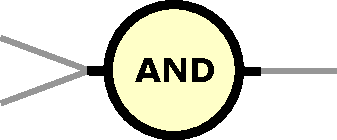
\includegraphics[scale = 0.5]{le_images/and}
  \caption{The \PD glyph for \glyph{and}. Only two inputs are represented, but more would be allowed.}
  \label{fig:and}
\end{figure}

%%%%%%%%%%%%%%%%%%%%%%%%%%%%%%%%%%%%%%%%%%%%%%%%%%%%%%%%%%%%%%%%%%%%%%
%%                     Or
%%%%%%%%%%%%%%%%%%%%%%%%%%%%%%%%%%%%%%%%%%%%%%%%%%%%%%%%%%%%%%%%%%%%%%
\subsubsection{Glyph: \glyph{Or}}\label{sec:or}

The glyph \glyph{or} is used to denote that any of the \glyph{EPNs} linked as input is sufficient to produce the output. \glyph{Or} is represented by a circle carrying the word ``OR''.

\begin{figure}[H]
  \centering
  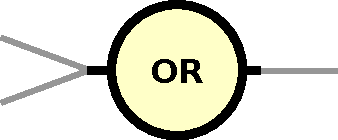
\includegraphics[scale = 0.5]{le_images/or}
  \caption{The \PD glyph for \glyph{or}. Only two inputs are represented, but more would be allowed.}
  \label{fig:or}
\end{figure}


%%%%%%%%%%%%%%%%%%%%%%%%%%%%%%%%%%%%%%%%%%%%%%%%%%%%%%%%%%%%%%%%%%%%%%
%%                     Not
%%%%%%%%%%%%%%%%%%%%%%%%%%%%%%%%%%%%%%%%%%%%%%%%%%%%%%%%%%%%%%%%%%%%%%
%\color{blue}
\subsubsection{Glyph: \glyph{Not}}\label{sec:not}

The glyph \glyph{not} is used to denote that the \glyph{EPN} linked as input cannot produce the output. \glyph{Not} is represented by a circle carrying the word ``NOT''.

\begin{figure}[H]
  \centering
  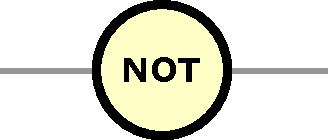
\includegraphics[scale = 0.5]{le_images/not}
  \caption{The \PD glyph for \glyph{not}.}
  \label{fig:not}
\end{figure}



%%%%%%%%%%%%%%%%%%%%%%%%%%%%%%%%%%%%%%%%%%%%%%%%%%%%%%%%%%%%%%%%%%%%%%
%%%%%%%%%%%%%%%%%%%%%%%%%%%%%%%%%%%%%%%%%%%%%%%%%%%%%%%%%%%%%%%%%%%%%%
%%%%                   Compartments
%%%%%%%%%%%%%%%%%%%%%%%%%%%%%%%%%%%%%%%%%%%%%%%%%%%%%%%%%%%%%%%%%%%%%%
%%%%%%%%%%%%%%%%%%%%%%%%%%%%%%%%%%%%%%%%%%%%%%%%%%%%%%%%%%%%%%%%%%%%%%
%
% %\section{Container nodes}\label{sec:CNs}
% \section{Representing compartments}
% Title not necessary since only one section

%%%%%%%%%%%%%%%%%%%%%%%%%%%%%%%%%%%%%%%%%%%%%%%%%%%%%%%%%%%%%%%%%%%%%%
%%%%                   Compartment
%%%%%%%%%%%%%%%%%%%%%%%%%%%%%%%%%%%%%%%%%%%%%%%%%%%%%%%%%%%%%%%%%%%%%%

\subsection{Glyph: \glyph{Compartment}}\label{sec:compartment}

A compartment is a logical or physical structure that contains entity pool nodes. An \glyph{EPN} can only belong to one compartment. Therefore, the ``same'' biochemical species located in two different compartments are in fact two different ``pools'' and should be represented by two \glyph{EPNs}.  A compartment is represented by a surface enclosed in a continuous border or located between continuous borders. These borders should be noticeably thicker than the borders of the \glyph{EPNs}. A compartment can take \textbf{any} geometry. A compartment must always be entirely enclosed.

\begin{figure}[H]
  \centering
  \includegraphics[scale = 0.3]{le_images/compartment}
  \caption{The \PD glyph for \glyph{compartment}.}
  \label{fig:compartment}
\end{figure}

To allow more aesthetically pleasing and understandable maps, compartments are allowed to overlap each other visually, but it must be kept in mind that this does not mean the top compartment contains part of the bottom compartment. 


% %%%%%%%%%%%%%%%%%%%%%%%%%%%%%%%%%%%%%%%%%%%%%%%%%%%%%%%%%%%%%%%%%%%%%%
% %%%%%%%%%%%%%%%%%%%%%%%%%%%%%%%%%%%%%%%%%%%%%%%%%%%%%%%%%%%%%%%%%%%%%%
% %%%%                   Submap
% %%%%%%%%%%%%%%%%%%%%%%%%%%%%%%%%%%%%%%%%%%%%%%%%%%%%%%%%%%%%%%%%%%%%%%
% %%%%%%%%%%%%%%%%%%%%%%%%%%%%%%%%%%%%%%%%%%%%%%%%%%%%%%%%%%%%%%%%%%%%%%
%
% \section{Submaps}
% Title not necessary since only one section

\subsubsection{Glyph: \glyph{Submap}}
\label{sec:submap}

A \glyph{submap} is used to encapsulate processes (including all types of nodes and edges) within one glyph.  The \glyph{submap} hides its content to the users, and display only input terminals (or ports), linked to \glyph{EPNs} (\sect{EPNs}). A \glyph{submap} is not equivalent to an \glyph{omitted process} (see \sect{omitted}).  
In the case of an SBGN description that is made available through a software tool, the content of a \glyph{submap} may be available to the tool.  A user could then ask the tool to expand the \glyph{submap}, for instance by clicking on the icon representing the \glyph{submap}.  The tool might then expand and show the \glyph{submap} within the same map (on the same canvas), or it might open it in a different canvas. In the case of an SBGN description made available in a book or a website, the content of the \glyph{submap} may be available on another page, possibly accessible via an hyperlink on the \glyph{submap}. 

The \glyph{submap} is represented as a square box to remind the viewer that it is fundamentally a process. A \glyph{submap} carries labeled terminals.  When the \glyph{submap} is represented folded, those terminals are linked to external \glyph{EPNs} (\sect{EPNs}).  In the unfolded view, exposing the internal structure of the \glyph{submap}, a set of \glyph{tags} point to the corresponding internal \glyph{EPNs} \sect{EPNs}. A \glyph{tag} is represented by a rectangle fused to an empty arrowhead. The symbol should be linked to one and only one edge (\ie it should reference only one EPN or compartment).

\begin{figure}[H]
  \centering
  \includegraphics[scale = 0.22]{le_images/submap}
  \caption{The \PD glyph for \glyph{submap}. (Upper part) folded submap. (Lower part) content of the submap. The \glyph{uncertain process} represents the content that is not available outside the submap.}
  \label{fig:submap}
\end{figure}

The left part of \fig{submap-folded} represents a \glyph{submap} that transforms glucose into fructose-6-phosphate. The \glyph{submap} carries five terminals, four linked to EPNs and one linked to a \glyph{compartment}.  The latter is particularly important in the case of EPNs present only in a \glyph{compartment} enclosed in a \glyph{submap}, and that are not linked to terminals themselves.  Note that the terminals do not define a ``direction'', such as input or output.  The flux of the reactions is determined by the context.

The map on the right of \fig{submap-folded} represents an unfolded version of the \glyph{submap}.  Here, anything outside the \glyph{submap} has disappeared, and the internal \glyph{tags} are not linked to the corresponding external \glyph{terminals}. The yellow nodes are also present in the parent map, while the salmon nodes are specific to the submap. Note the tag 5, linking the compartment ``mito'' of the \glyph{submap} to the compartment ``mito'' outside the \glyph{submap}.  The compartment containing Glu6P is implicitly defined as the same as the compartment containing Glu and Fru6P.  There is no ambiguity because if Glu and Fru6P were in different compartments, one of them should have been defined within the \glyph{submap}.

\begin{figure}[H]
  \centering
  \includegraphics[scale = 0.4]{le_images/submap-folded}
  \includegraphics[scale = 0.35]{le_images/submap-unfolded}
  \caption{Example of a submap with contents elided.}
  \label{fig:submap-folded}
\end{figure}


% \section{Referring to other Nodes}
%
% Reference nodes handle links or relationships between elements of a map and sub-map. At present there is only one reference glyph, \glyph{tag}, which can be used in a map refered to by a \glyph{submap} (\sect{submap}) or as an auxilary unit on the \glyph{submap}. The \glyph{clone marker} can also provide additional reference mechanisms and is discussed below (\sect{cloneMarker}).
%
% \subsection{Glyph: \glyph{Tag}}
\label{sec:tag}

A \glyph{tag} is a named handle, or reference, to another \glyph{EPN} (\sect{EPNs}) or \glyph{compartment} (\sect{compartment}) of the map.
Together with the \glyph{submap terminal} (\sect{submapTerminal}), it allows linking glyphs of a map to their counterpart in a submap.

\begin{glyphDescription}

\glyphSboTerm Not applicable.

\glyphIncoming
One \glyph{equivalence arc} (\sect{equivalenceArc}).

\glyphOutgoing
None.

\glyphContainer A \glyph{tag} is represented by a rectangular shape fused to an empty arrowhead, as shown in \fig{tag}.
The incoming \glyph{equivalence arc} (\sect{equivalenceArc}) should be linked to the extremity of the arrowhead.

\glyphLabel A \glyph{tag} is identified by a label that is  a string of characters that may be distributed on several lines to improve readability.
The centre of the label must be placed on the centre of the shape.
The label may extend outside of the shape.

\glyphAux 
None.

\end{glyphDescription}

\begin{figure}[H]
  \centering
  \includegraphics{images/build/tag.pdf}
  \caption{The \PD glyph for \glyph{tag}.}
  \label{fig:tag}
\end{figure}

%
%
%
\section{Building a SBGN \PDm}
\label{chp:build}

Now that the various symbols used by the SBGN \PDl have been introduced, some guidance on building map will be provided. 

\subsection{How to choose the symbols to use?}
\label{sec:choose}

It is important to realise that there are in general more than one way to represent a system in SBGN \PD. The choice of concepts and symbols often depend on the granularity of information available, and the message the authors of the map wish to convey to the readers of the map. 

As a first example of variable information granularity, let's take will take the example of MAP kinase phosphorylation (ERK). A very simple representation would be to encode the state of phosphorylation in \glyph{entity pools node} with different names, ERK, ERK-P, ERK-PP (\fig{MAPK-NoVar}).
 
\begin{figure}[H]
  \centering
  \includegraphics[scale = 1]{le_images/MAPK-NoVar}
  \caption{Phosphorylation of ERK by MEK, where ERK is represented by three different macromolecules.}
  \label{fig:MAPK-NoVar}
\end{figure}

This kind of representation would be obtained if the SBGN \PDm was generated from a model encoded in SBML core \cite{Hucka:2003}. One of the problems with this representation is the difficulty for the reader to understand that the effect of MEK is to catalyse the phosphorylation of ERK. A scientist familiar with signalling pathways would probably imediately make the connection. A biologist in general could be more cautious. ``P'' could represent anything (peptide? proline?). A computer would require a special algorithm to parse the names, and this algorithm would easily fail. Instead of ERK-PP, we could have used PP-ERK, ERK\_PP, ERKP1P2, ERKTPYP etc. But in fact, there is nothing in the the map \fig{MAPK-NoVar} indicating that the reactions catalysed add covalent modifications to ERK. Thore reactions could be anything, such as aggregation, cleavage etc.

In order to overcome those issues, one can use state variables. On \fig{MAPK-OneVar}, one uses a single state variables to represent the number of phosphorylations on ERK. 

\begin{figure}[H]
  \centering
  \includegraphics[scale = 1]{le_images/MAPK-OneVar}
  \caption{Phosphorylation of ERK by MEK, where ERK is represented by three different states, non-phosphorylated, mono-phosphorylated and bi-phosphorylated.}
  \label{fig:MAPK-OneVar}
\end{figure}

Because 'P' is a reserved symbol of the covalent modifications vocabulary, there is no ambiguities. We know that each reaction add a phosphate to ERK. That would be the representation to favour if we only know the number of phophorylation (e.g. by western blot with non-specific antibodies), or if we do not care which site is phosphorylated. Note that the leftmost ERK carries an empty state variable, that is equivalent to ``0P''. The state variable is not ommited. This rule of \SBGNPDLone is called ``once a variable, always a variable'' (OVAV).
If we want to, or can, be more specific about distinct phosphorylations, one can create two state variables, one for each site (\fig{MAPK-TwoVar}). 

\begin{figure}[H]
  \centering
  \includegraphics[scale = 1]{le_images/MAPK-TwoVar}
  \caption{Phosphorylation of ERK by MEK, where each phosphorylated form of ERK is represented.}
  \label{fig:MAPK-TwoVar}
\end{figure}

In this representation, we have all the information related to the two phosphorylation sites, the threonine and the tyrosine. They are represented by the variable symbols T and Y in the figure. But one could have chosen X and Y or 1 and 2. The important issue is to distinguish them. Note that the creation of an extra \glyph{entity pool node} is unavoidable. \SBGNPDLone does not currently allow logical expressions in the state variables. Therefore if only one \glyph{entity pool node} was to be used to represent the single-phosphorylated form, a choice between T or Y should have been made, and the resulting map would not have carried the same information than  (\fig{MAPK-OneVar}).

% complex: macromolecule or complex
As a second example, we will consider the oxygenation of hemoglobin. If one wants to convey the message that 4 oxygene molecules bind to a molecule of hemoglobin, it is sufficient to create \glyph{macromolecules} for hemoglobin and oxy-hemoglobin. 

\begin{figure}[H]
  \centering
  \includegraphics[scale = 0.4]{le_images/hemoglobin-macromolecule}
  \caption{Hemoglobin oxygenation using \glyph{macromolecules}.}
  \label{fig:hemoglobin-macromolecule}
\end{figure}

If conveying the fact that hemoglobin is a multimer is important (for instance to suggest cooperativity), one can use \glyph{multimers} instead. In addition, in \fig{hemoglobin-multimer}, the concept of oxygenation is represented with a state variable rather than being embedded in the name of the nodes.

\begin{figure}[H]
  \centering
  \includegraphics[scale = 0.4]{le_images/hemoglobin-multimer}
  \caption{legend}
  \label{fig:hemoglobin-multimer}
\end{figure}

An additional layer of complexity is needed if we want to mention the $\alpha$ and $\beta$ subunits. A \glyph{complex} can then be used. In addition \fig{hemoglobin-complex} explicitely represent the complexes between globin and oxygene instead of using state variables.

\begin{figure}[H]
  \centering
  \includegraphics[scale = 0.4]{le_images/hemoglobin-complex}
  \caption{legend}
  \label{fig:hemoglobin-complex}
\end{figure}

In conclusion, one can see that many different choice are offered to represent an idea in SBGN, and the map writers make the choice. By doing so, they acknowledge that more or less information can be extracted from the resulting map. The important issue is that anyone reading the map interpret it the same way. That is the topic of the following section. 

